\chapter{Magnitude History, Productivity Sensitivity, Exposure Orthogonalization, and Kernel Refinements}
\label{ch:temporal-extensions}\label{chap:temporal-extensions}
The historical observed comparison is retained in Chapter~\ref{ch:observed}.
This chapter consolidates the separately frozen magnitude-history and
productivity studies, followed by exposure orthogonalization, parent-class
temporal scales and continuously tuned Omori triggering. Each comparison uses
its own matched reference. The same historical targets recur across sensitivity
settings; they do not become independent replications.

This reuse is sequential and adaptive at programme level: inspected results helped motivate later model families, parameter domains and reporting contrasts. A protocol frozen before one stage constrains that stage's execution but does not restore an unused holdout after earlier inspection. The resulting scores are exploratory comparisons on a shared archive, subject to the adaptive-data-analysis distinction discussed by \citet{Dwork2015}.

For the temporal models, $P=Q$, timing is $Q+C$, and the joint marked score is
$P+C+M$, with $E>0$ integrated exposure and $C=-E$. Reported differences are
candidate minus the named reference. The source reports' event field (sometimes
called $E$ historically) is displayed here as $\Delta Q$; their compensator
contrast is $\Delta C$. The magnitude excess $q=M_{\rm magnitude}-5$ must not
be confused with the score component $M$. The class cutoff denoted $c$ in the
class-history equations is $c_{\rm class}=0.5$ magnitude units, whereas $c$
in the Omori sections is a temporal scale in days. These are separate local
namespaces. The free-productivity coordinate is continuous on $[0,0.95]$;
the seven-node grid below is a descriptive profile, not its optimization domain.


\section{The earlier magnitude-history misspecification pilot}
\label{sec:magnitude-history-pilot}
The run \path{magnitude_history_20261023T205716Z} precedes the observed
class-history forecast investigation. It asks whether changing magnitude
dependence alters a preserved inhibitory fitting procedure's preference under
a designed, entirely excitatory generating family. It is neither a fitted
comparison of the richer excitatory family nor a forecast experiment.

For magnitude excess $q$ with exponential rate $b$ and bin cutoff $a_{\rm bin}$, let $p_0=1-e^{-b a_{\rm bin}}$ and $p_1=e^{-b a_{\rm bin}}$. The bins are $[0,a_{\rm bin})$ and $[a_{\rm bin},\infty)$. Let
$P_{ij}(h)=(1-h)p_i+h\mathbf1_{i=j}$. With common normalized waiting density
$k$ and no magnitude productivity in the generator,
\[
 \lambda_i(t)=\mu p_i+n_g\sum_{k:t_k<t}P_{iJ_k}(h)k(t-t_k),\qquad
 \Lambda(t)=\mu+n_g\sum_{k:t_k<t}k(t-t_k).
\]
Generate the untyped timed branching forest first. Since the columns of $P$
sum to one and $Pp=p$, assigning immigrant classes from $p$ and child classes
from the parent's column preserves each node's marginal class law by induction.
Fixed-window censoring and chronological ordering depend only on the untyped
forest, so this remains an exact finite-window statement conditional on the
entire timed forest and its event count. Mixing the exponential law restricted
to each bin recovers exactly the same exponential one-event magnitude law.
At $h=0$ the marks are iid; positive $h$ changes labelled-history dependence
without changing total timing or one-event marginals. Class counts at positive
$h$ need not be multinomial, and conditioning on label-selected subsets does
not preserve this argument. In particular, with class histories $S_i$ and
$S=\sum_iS_i$,
\[
 \frac{\lambda_i}{\Lambda}
 =p_i+\frac{n_gh}{\Lambda}(S_i-p_iS).
\]
Each absolute class intensity is nonnegative and receives nonnegative event
increments even though its conditional class probability can decrease.

The same timed forest is labelled under all three persistence scenarios using
fixed per-node random inputs and separate time/mark streams. The independent
replicate is the forest, not each scenario catalogue or each event. The old
candidate uses magnitude-productivity exponent $r=0.7$, whereas the generator has no magnitude productivity ($r=0$, or $\gamma=0$ in its parameterization). Its finite-mixture temporal representation also differs from exact Mittag-Leffler generation. The candidate therefore remains misspecified even
at $h=0$; the mismatches are common across scenarios. Supplied-background
settings do not become true generator parameters. Positive nested fit gains
therefore cannot be interpreted as calibrated false-positive rates.

\subsection{Generator settings and fitted statistic}

The generator is a designed two-class MDFHP-form excitatory family with common Mittag-Leffler shape $0.5$ and scale $1/\mathrm{day}$, total immigrant rate $\exp(-4.162108473051707)$, offspring mean $0.5$ and empty prehistory over 24,394 days. Magnitude excess has marginal exponential rate $2.849401764894274$, with bins $[0,0.5)$ and $[0.5,\infty)$. The $\gamma=0$ productivity boundary and unbounded final bin are explicit extensions of the published fitted specification.
Selection was frozen as direct $\mathrm{GLR}>0.001$ and selected $\eta>\text{\texttt{1e-6}}$. No Wilks reference law, calibrated rejection cutoff, power ranking or physical-mechanism interpretation was used.

For scenario $h$ and planned independent skeleton $s$, let $G(s,h)$ be the procedure's resolved direct likelihood-ratio statistic and $\eta(s,h)$ its selected inhibition parameter. The frozen descriptive preference indicator equals $1$ when $G$ exceeds $0.001$ and $\eta$ exceeds $\text{\texttt{1e-6}}$. These thresholds define an operational preference; they are not calibrated significance cutoffs. The primary contrasts compare the preference indicator and continuous statistic at positive $h$ with the matched baseline at $h=0$ on the same skeleton.

Every scenario's planned denominator is retained. Resolved-only frequencies estimate a resolution-conditional descriptive quantity, with its denominator stated. If $k$ cases select inhibition and $u$ cases are unknown out of $N$ planned cases, the all-planned selection frequency is bounded by $[k/N,(k+u)/N]$. These are missing-outcome accounting bounds, not confidence intervals. Continuous-statistic summaries based on resolved cases remain conditional summaries; missing continuous values are not replaced by zero.

The frozen persistence values are $h=0$, $0.5$ and $0.9$. The actual pilot kernel has Mittag-Leffler shape $0.5$ and inverse-time scale $c=1\,\mathrm{day}^{-1}$, corresponding to the time scale $1/c=1$ day. This pilot $c$ is distinct from the Omori time scale used later in this chapter. The independent compiled core supports only shape $0.5$ and $1$; support for another shape is not claimed. Here $b$ is the continuous mark rate and $n_g$ is the generator branching mean. They are distinct from similarly named shape/productivity parameters in the preserved comparison engine.

The frozen primary procedure estimates background level and trend together with the inhibition alternative, while retaining the staged procedure's supplied triggering, stress and mark-rate settings. Its prescribed starts comprise two null fits followed by two alternative starts from the selected null. A secondary supplied-background procedure uses two inhibition starts. The supplied-background label does not mean its nuisance settings are true generating parameters.

This source-bound six-start staged comparison is narrower than the historical full kernel/productivity searches, the separate later nuisance continuation or the observed-catalogue fitting recipe. Results must identify this exact procedure. They cannot be substituted into historical counts, reference banks or claims about the larger searches. Solver starts, explicit $\eta=0$ eligibility, subset floors, failure-only recovery and original numerical controls remain part of the procedure. Local optimization is not a global optimum certificate.

The $h=0$ scenario is the experiment's independence baseline, not an in-model null-size experiment for the old procedure. The generator has $\gamma=0$ magnitude productivity, while the old candidate intensities depend on prior continuous marks through their productivity and stress transforms. Exact Mittag-Leffler generation and the old finite-mixture representation also remain distinct. These mismatches are common to the persistence scenarios; the paired persistence contrast isolates the change in magnitude history within this deliberately specified stress family, without establishing correct specification at $h=0$.

The primary comparison uses the same realized continuous marks and exposure for its excitatory and inhibitory candidates. A common mark-density term can cancel within that paired comparison, but marks still enter subsequent candidate intensities. Dropping a common density term does not justify discarding the marks. No comparison of raw continuous densities with discrete bin masses is made, and no held-out forecast-score claim follows from these fitted-statistic preferences.

\subsection{Pairing, numerical exposure and reproducibility limits}

The plan contains 20 independent untyped skeletons, each labelled under all three persistence scenarios. There are 60 scenario catalogues but 20 independent replicate blocks. Pairing shares the untyped skeleton and fixed per-node random inputs, while each scenario generates its own conditional labels and within-bin magnitudes. One fixed iid mark sequence must not be reused as the observed marks in every scenario.

Separate time and mark pseudorandom streams, their exact implementation, the compiler and runtime are pinned. Equal seeds in another language or standard-library implementation are not asserted to reproduce the same streams. Uncertainty for persistence contrasts resamples skeleton blocks. Resolved-only paired contrasts state the number of paired-resolved skeletons; all-planned bounds additionally retain unknown preference indicators. Pilot intervals are exploratory Monte Carlo summaries, not confirmatory coverage certification.

The synthetic window is fixed independently of the first and last events. The likelihood retains initial quiet exposure, every positive event gap and the final no-event interval. Saved two-part timestamps and positive gaps define ordering, including cases where a lossy binary64 projection ties. The generator reports a precision failure when its declared parent-child wait-error gate is exceeded; it does not redraw a wait, jitter an event or replace a magnitude to force completion. Resource caps and unresolved mandatory solver states stay explicit unknown outcomes.

The computational route combines an independently implemented C++ generator/numerical core, an R interface and the preserved Python comparison machinery with its declared CUDA/FP64 primary route and existing failure-only recovery. It is not a full rewrite of the historical engine. Independent mathematical/spectral-quadrature, saved-clock and waiting-law controls have separate evidence and declared finite scopes.

An additional reference bridge ran the original released ml.m in GNU Octave. A private byte-preserving copy changed only the C++ dispatch switch to select its original language implementation; the copyright notice and original clone were retained. Fixed-input survival and kernel calculations were compared against the new independent core. This is executable original-source validation without MATLAB, not reproduction of the original MATLAB optimizer, all fitted examples or every numerical regime.

The exact author preprint is separately pinned from the version of record. The exact published supplement remains unavailable in this run, the released Japan CSV contains no event rows, and historical banks excluded from the existing public package remain unavailable. Those gaps constrain exact-reproduction claims; they do not authorize reconstructing historical inputs by guesswork. Third-party source copies and raw catalogue material are not covered by a blanket project licence and remain outside a tidy public payload unless their terms are established.

$\gamma=0$ is a boundary/limiting case of the released positive-productivity fitting transform. The unbounded final magnitude bin extends the article's finite upper magnitude support. The accurate model label is a designed MDFHP-form excitatory stress family with matched exponential marginal marks, not an exact recovered author fit or the entire MDFHP family.

No correctly specified richer excitatory model is fitted in this bounded pilot. A changed inhibitory preference would demonstrate a vulnerability or response of the selected old procedure under this generator; it would not establish that an estimated MDFHP practically absorbs the effect in observed data. Conversely, a small or unresolved contrast would be limited to this family, sample budget and fitting procedure; it would not rule out other magnitude-history mechanisms.

There is no fresh null calibration, size-matched power comparison, observed-catalogue evaluation, causal intervention or physical inhibition identification. Pointwise checks cannot establish uniform performance over nuisance parameters. No combined inhibitory MDFHP, general exact-memory stability theorem, exhaustive novelty claim or external-publication conclusion is asserted. Final claims require terminal saved outputs, complete failure accounting and independent review.

\section{Historical pilot results and interpretation}

The validated machinery is feasible, and the full bounded pilot completed: 20 independent timed forests, three magnitude-dependence scenarios, 60 catalogues and 120 resolved method outcomes. No planned outcome is missing.

Under the frozen descriptive rule, the primary fitted-background comparison preferred positive inhibition in 15/20 independent-mark controls, 17/20 moderate-dependence histories and 18/20 strong-dependence histories. However, both primary paired GLR-difference intervals span zero. This pilot does not establish a clear increase in likelihood evidence specifically caused by magnitude history, or explain previous observed-catalogue evidence.

A nested, unpenalized alternative can improve fit under an excitatory generator. The rule below resolves a positive fit preference near numerical tolerance; these frequencies are not calibrated false-positive rates and do not demonstrate failure of any advertised calibrated inhibition test.

\subsection{Complete outcomes}

All 20 cases per scenario resolved, so resolution-conditional and all-planned frequencies coincide here. Wilson intervals describe Monte Carlo selection frequencies under this rule. They do not calibrate the test. Missing-outcome bounds are retained in the machine-readable summary and are not confidence intervals.
{\small
\setlength{\tabcolsep}{3pt}
\begin{longtable}{llrrrrr}
\caption{All six descriptive pilot frequency cells. Wilson endpoints are frequency fractions across independent forests; they do not calibrate the inhibitory test.}\label{tab:pilot-frequency}\\
\toprule
Procedure & $h$ & Selected/planned & Unknown & Wilson lower & Wilson upper & Median GLR\\\midrule
\endfirsthead
\toprule
Procedure & $h$ & Selected/planned & Unknown & Wilson lower & Wilson upper & Median GLR\\\midrule
\endhead
Supplied & 0.0 & 6/20 & 0 & 0.145477 & 0.518973 & 0.000000\\
Supplied & 0.5 & 6/20 & 0 & 0.145477 & 0.518973 & 0.000000\\
Supplied & 0.9 & 4/20 & 0 & 0.080658 & 0.416017 & 0.000000\\
Fitted (primary) & 0.0 & 15/20 & 0 & 0.531299 & 0.888138 & 1.205812\\
Fitted (primary) & 0.5 & 17/20 & 0 & 0.639581 & 0.947631 & 1.053431\\
Fitted (primary) & 0.9 & 18/20 & 0 & 0.698966 & 0.972134 & 1.052331\\
\bottomrule
\end{longtable}
}

\subsection{Paired changes from the independent-mark control}

Each contrast uses all 20 paired forests and the predeclared 20,000-resample skeleton bootstrap, seed 2026102499. These are exploratory percentile summaries, not confirmatory coverage guarantees. A zero or zero-touching interval is not proof of equivalence.

The primary selection frequency rises, but its median GLR does not increase and its paired mean GLR changes are small relative to their uncertainty. The secondary procedure moves in the opposite direction at strong persistence. These observations do not support a simple, procedure-independent claim that stronger magnitude history yields stronger inhibitory evidence.

The post-execution class-manipulation diagnostic is recorded separately in methods/pilot\_input\_diagnostics.json: observed parent-child same-class fractions were approximately 0.6304, 0.8207 and 0.9656, versus design expectations 0.6346, 0.8173 and 0.9635. This is a descriptive implementation diagnostic, not a new primary test; no event-iid uncertainty is asserted.

\noindent The pilot implementation, validation and resources are retained in \hyperref[app:audit09-pilot-implementation]{Appendix~\ref{app:audit09-pilot-implementation}}.
{\small
\setlength{\tabcolsep}{3pt}
\begin{longtable}{llrrrrrr}
\caption{All four paired changes from the independent-mark control. Selection changes are frequency fractions (multiply by 100 for percentage points); endpoints are exploratory paired-forest bootstrap summaries, not confirmatory coverage.}\label{tab:pilot-paired}\\
\toprule
Procedure & $h$ & Selection diff. & Lower & Upper & GLR diff. & Lower & Upper\\\midrule
\endfirsthead
\toprule
Procedure & $h$ & Selection diff. & Lower & Upper & GLR diff. & Lower & Upper\\\midrule
\endhead
Supplied & 0.5 & 0.000000 & 0.000000 & 0.000000 & -0.010306 & -0.039395 & 0.018140\\
Supplied & 0.9 & -0.100000 & -0.250000 & 0.000000 & -0.040430 & -0.073392 & -0.012346\\
Fitted (primary) & 0.5 & 0.100000 & 0.000000 & 0.250000 & -0.162155 & -0.846990 & 0.354902\\
Fitted (primary) & 0.9 & 0.150000 & 0.000000 & 0.300000 & 0.030885 & -1.114732 & 1.029795\\
\bottomrule
\end{longtable}
}

\begin{figure}[tbp]
\centering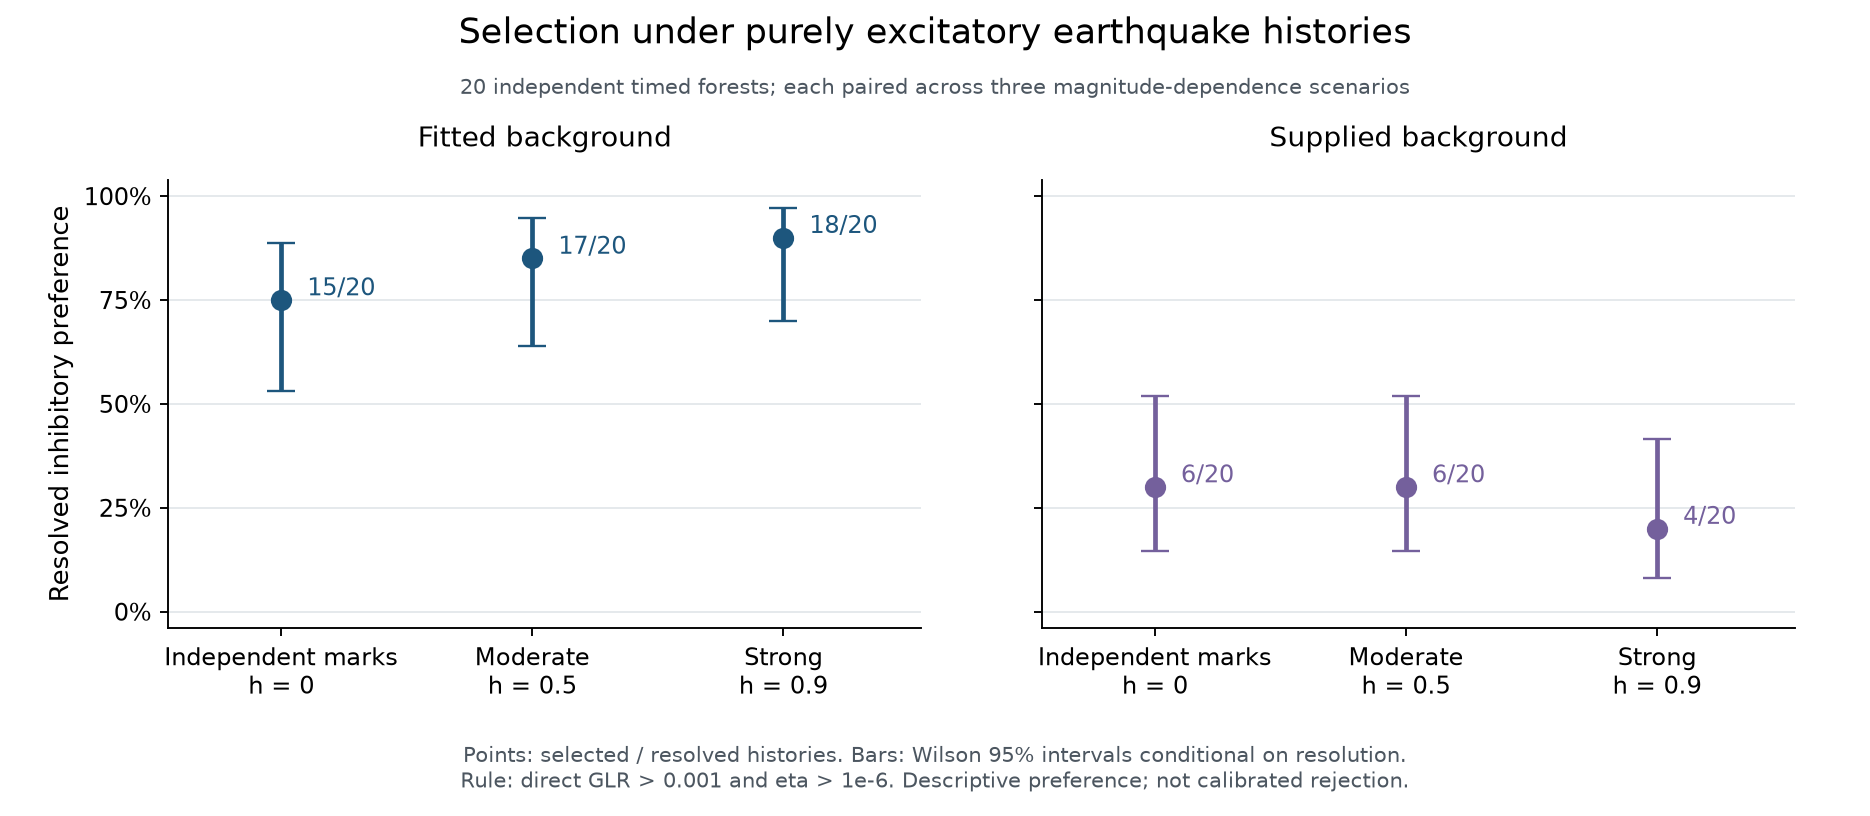
\includegraphics[width=\linewidth]{a2_pilot_selection_final.png}
\caption{Saved final magnitude-history pilot selection frequencies. Forests
are paired across scenarios. These descriptive Monte Carlo intervals do not
calibrate a rejection test or establish a magnitude-history mechanism.}
\label{fig:magnitude-history-pilot}
\end{figure}

\subsection{Interpretation}

The feasibility and bounded descriptive pilot gates pass. The machinery can generate the intended history-dependent marks and apply the selected existing comparison reproducibly. The completed observation is that this narrow procedure can show positive inhibitory fit preference under a purely excitatory designed family, including its independent-mark control.

Whether accounting for magnitude history explains previous observed evidence remains unresolved. No correctly specified richer excitatory model was fitted in this cycle; known-law scoring controls are separate from fitting. There was no fresh null calibration, size-matched power comparison, observed-catalogue evaluation or held-out forecast comparison.

The next scientific stage should first define the claim and fit the competing excitatory family under a reviewed protocol, while separating common productivity misspecification from the history contrast. Any advertised rejection test then needs fresh calibration and independent evaluation banks reproducing nuisance fitting and selection. An observed-data comparison would require matched scoring targets/exposure and separate catalogue/completeness gates. No additional campaign was launched here.

\noindent The pilot reproducibility artifacts are retained in \hyperref[app:audit09-pilot-artifacts]{Appendix~\ref{app:audit09-pilot-artifacts}}.

\noindent The pilot evidence map is retained in \hyperref[app:audit09-pilot-evidence]{Appendix~\ref{app:audit09-pilot-evidence}}.

\section{Purpose and relationship to the earlier releases}
\label{a2:purpose}

The original GitHub research manuscript separates mathematical legitimacy,
identification of an observation law and the predictive value of a fitted
procedure (Chapter~\ref{ch:observed}; Appendix~\ref{app:custody}). Its first addendum examined a separate
background-nuisance continuation whose initial null gap is closed in
Section~\ref{sec:f-continuation} (Appendix~\ref{app:custody}). This second companion adds a different empirical
axis: whether magnitude-class history or a more flexible magnitude-productivity
law improves the declared predictive comparisons. It reports the two completed
follow-ups, their numerical evidence and their stopping decisions, preserving
the earlier scientific records.

The distinction between releases is substantive. The manuscript's observed
reconstruction selected productivity ratios \(r=0.4,0.7,0.7\) at its three
origins. The new matched reference candidates use \(r=0.7\) throughout and a
different, common training-only magnitude-rate estimator
(Table~\ref{a2:recipe}). They are separately specified follow-up experiments,
not replacements for the manuscript's historical score table. Both use the
same hash-pinned GeoNet selection as our observed reconstruction. That archive
identity does not establish identity with the unavailable earlier analysis
discussed in the manuscript's catalogue-provenance section.

\begin{table}[tbp]
\centering\small
\caption{Scientific lineage and recipe differences. These studies are
related releases, not interchangeable fits or pooled calibration results.}
\label{a2:recipe}
\begin{tabular}{>{\raggedright\arraybackslash}p{0.18\linewidth}>{\raggedright\arraybackslash}p{0.34\linewidth}>{\raggedright\arraybackslash}p{0.39\linewidth}}
\toprule
Study & Question/target & Productivity and magnitude treatment\\
\midrule
Original manuscript &
Restricted stability/identification, controlled nuisance comparisons,
and exploratory observed prediction &
Observed recipe selected \(r=0.4,0.7,0.7\) at the three origins;
training plug-in magnitude rates \(3.101622\), \(3.149488\), \(3.021907\).\\
F companion &
Four-procedure synthetic background-nuisance continuation; old null
gap resolved in Stage~2 &
Supplied triggering/mark law in the declared nuisance comparison;
its counts and procedure differ from the historical study.\\
Class-history follow-up &
Does a restricted class-history extension improve matched forecasts? &
Fixed \(r=0.7\); shared training-only conditional-bin magnitude
estimator; source fertility \(\delta\) and association \(h\).\\
Productivity follow-up &
Does a training-estimated continuous slope improve matched forecasts? &
Same conditional-bin magnitude estimator;
fixed \(r=0.7\) versus estimated \(r\in[0,0.95]\) in E0 and I0;
class-history continuation gated off.\\
\bottomrule
\end{tabular}
\end{table}


\subsection{External framework and attribution}

Self- and mutually exciting point processes provide a natural setting for
event-triggered clustering \citep{Hawkes1971}; earthquake triggering models
include the ETAS tradition \citep{Ogata1988}. Davis, Baeumer and Wang's
fractional earthquake model supplies context for Mittag-Leffler triggering
with magnitude productivity \citep{DavisBaeumerWang2024}. Their multivariate
fractional construction represents magnitude ranges as subprocesses and
permits history-dependent magnitude proportions
\citep{DavisBaeumerWang2026}. We inspected its model definitions in the
separately identified author preprint, Section~2, equations~(2)--(4)
\citep{DavisBaeumerWangPreprint2024}; those locators do not assert final-journal
pagination. For positive linear marked Hawkes models, partitioned multivariate
constructions provide an approximating parametric description under stated
assumptions \citep{DavisKresinBaeumerWang2026}. No stationarity or
identification theorem from that setting is transferred to our nonlinear
inhibitory comparator. These sources motivate the question and
model language; they do not supply the empirical findings reported here.

Our low-dimensional two-class shared-kernel family simplifies some class
and kernel structure while changing mark support and nuisance treatment.
The consulted MDFHP preprint \citep[Section~2]{DavisBaeumerWangPreprint2024}
uses truncated within-bin magnitude densities, including an upper magnitude
of 10. Our working exponential excess law is
unbounded. Consequently, our complete joint model is not a strict submodel
of that specification. The present comparisons neither reproduce nor refute
the authors' Japan and Middle America fitted results. Their results and
software must be credited in their own scope, and the locally derived
summation identity below is a result for the family actually implemented.

\section{Restricted class history and productivity sensitivity}
\label{a2:models}

The class-history candidate is a restricted two-class, shared-kernel
construction motivated by multivariate representations of marked excitation
\citep{DavisBaeumerWang2026,DavisKresinBaeumerWang2026}.
The equations below specify the implemented follow-up family; they are not
the full fitted model or a reproduction of the empirical comparisons in those
papers. It simplifies class and temporal-kernel structure while changing the
mark support, and is not a strict submodel of the authors' bounded-mark
family. Shared target kernels and the low-dimensional association parameter
are choices of this experiment. Notation is local: our \(\beta\) denotes the
magnitude rate, rather than a source paper's fractional-kernel order.

\subsection{Class association and the conditional ground intensity}

Write \(q=M-5\), let the class cut be \(c=0.5\), and define
\(\mathcal C_0=[0,c)\), \(\mathcal C_1=[c,\infty)\). Write
\(p_0=1-e^{-\beta c}\), \(p_1=e^{-\beta c}\) for the background class
probabilities under the working excess-exponential law. The common
\(\beta>0\) is estimated using training marks only and held fixed in each
forecast window. Let \(C_k\in\{0,1\}\) be the class label of event \(k\).
For source class \(j\), define the strictly past history
\[
 H_j(t)=\sum_{k:\,t_k<t,\ C_k=j}\kappa_{0.7}(q_k)g(t-t_k),
 \qquad
 R_0(\delta)=e^{-\delta/2},\quad R_1(\delta)=e^{\delta/2},
\]
where \(g\) is the retained unit-integral finite positive exponential
mixture and \(\kappa_r\) is defined in equation~\eqref{a2:productivity}.
Write \(\mu(t)=\exp\{a+d x_{\mathrm{trend}}(t)\}\) for the background, with the affine
observation coordinate specified in Section~\ref{a2:protocol}.
The implemented target-class intensity is
\begin{equation}
 \begin{aligned}
 \lambda_i(t)&=p_i\mu(t)+\frac{n}{\rho(h,\delta)}
       \sum_{j=0}^1 P_{ij}(h)R_j(\delta)H_j(t),\\
 P_{ij}(h)&=(1-h)p_i+h\,\mathbf 1_{\{i=j\}}.
 \end{aligned}
 \label{a2:class-intensity}
\end{equation}
Here \(n\) is the class-history candidate's scalar branching parameter and
\(\rho(h,\delta)\) is the normalizing Perron root specified below.
The frozen parameter box is
\[
 -0.95\min(p_0/p_1,p_1/p_0)\leq h\leq 0.95,\qquad
 -1\leq\delta\leq1,\qquad 0\leq n\leq 0.98.
\]
The factor \(0.95\) retains a margin inside the mathematical
nonnegativity limit for \(P\); the Perron root \(\rho(h,\delta)\) is
strictly positive.
For the working within-class magnitude laws, let
\[
 m_j=E[\kappa_{0.7}(Q)\mid Q\in\mathcal C_j],\qquad
 m_0=\frac{1-e^{-0.3\beta c}}{p_0},\quad m_1=e^{0.7\beta c}.
\]
The raw mean offspring matrix and its normalization are
\[
 A_{ij}(h,\delta)=P_{ij}(h)R_j(\delta)m_j,\qquad
 \rho(h,\delta)=\rho_{\rm PF}(A),\qquad K=\frac{n}{\rho}A,
\]
where \(\rho_{\rm PF}\) denotes the Perron root. Thus \(K\) is the
class-history candidate's mean offspring matrix, with Perron radius \(n\).
Association \(h\) and fertility contrast \(\delta\) play different roles.
Signed association can describe class anti-persistence while all
excitation coefficients remain nonnegative. At \(n=0\),
\(\lambda_i=p_i\mu\); trigger association and fertility are unidentified.

For every source class, \(\sum_iP_{ij}(h)=1\). Thus, conditional on a
fixed observed marked history,
\begin{equation}
 \Lambda(t)=\sum_i\lambda_i(t)
 =\mu(t)+s\{R_0(\delta)H_0(t)+R_1(\delta)H_1(t)\},
 \qquad s=\frac{n}{\rho(h,\delta)}.
 \label{a2:ground-intensity}
\end{equation}
The direct redistribution across target classes cancels from the ground
intensity. The conditional timing log likelihood is
\[
 \ell_{\rm time}=\sum_k\log\Lambda(t_k)-\int_{\mathcal W}\Lambda(t)\,dt.
\]
For these classes, the conditional within-class magnitude density is
\[
 f_i(q)=\frac{\beta e^{-\beta q}}{p_i}\mathbf1_{\{q\in\mathcal C_i\}}.
\]
The mark density at an observed event of class \(i\) is
\(\{\lambda_i(t)/\Lambda(t)\} f_i(q)\), giving mark log density
\(\log(\lambda_i/\Lambda)+\log\beta-\beta q-\log p_i\).
This gives the saved decomposition
\(\ell_{\rm joint}=\ell_{\rm time}+\ell_{\rm mark}\).

Equation~\eqref{a2:ground-intensity} has several qualifications.
First, holding \(n\) fixed does not remove \(h\), because \(\rho\) may
depend on \(h\). Second, matching an effective scale at \(h=0\) requires
\[
 n_0=n\frac{\rho(0,\delta)}{\rho(h,\delta)}.
\]
This mapping preserves timing intensities only if the mapped parameter is
admissible, in particular \(0\leq n_0\leq 0.98\); \(n=0\) gives the
trivial no-trigger case. The frozen bound on \(n\), and any relevant
stability constraint, can make feasible effective-scale ranges depend on
\(h\). We therefore do not assert that all constrained timing families are
identical. Third, joint timing-and-mark estimation can shift \(s,\delta\)
and background parameters, producing indirect changes in timing forecasts.
Finally, the identity conditions on the actually observed marked past.
When future marks themselves are generated by the model, their class
composition can depend on \(h\), and so can a multistep or unconditional
timing law.

At \(h=0\), \(\lambda_i(t)=p_i\Lambda(t)\); the conditional magnitude law
is history-free even when \(\delta\) remains fitted. Consequently, we denote this association-zero ablation \(E1_{h=0}\);
it is the appropriate primary ablation for the association parameter
within this restricted family. It is not the same restriction
as setting both \(h\) and \(\delta\) to zero.

\subsection{Continuous productivity and dynamic evaluation}

The second follow-up replaces fixed \(r=0.7\) by a training-estimated
\(r\in[0,0.95]\) in
\begin{equation}
 \kappa_r(q)=(1-r)e^{\beta rq},\qquad
 \partial_r\kappa_r(q)=\kappa_r(q)
            \left(\beta q-\frac{1}{1-r}\right).
 \label{a2:productivity}
\end{equation}
For \(Q\sim{\rm Exp}(\beta)\), \(E[\kappa_r(Q)]=1\) when \(r<1\).
This is a normalization under the working law, not an empirical statement
about the historical magnitude catalogue.

The geometry records \(D_{ik}=g(t_i-t_k)\mathbf 1_{\{t_k<t_i\}}\)
and each parent's full-window exposure \(J_k\), independently of \(r\).
Every C++ value and gradient evaluation recomputes
\[
 H_r(t_i)=\sum_k D_{ik}\kappa_r(q_k),\quad
 K(r)=\sum_kJ_k\kappa_r(q_k)
\]
and their \(r\)-derivatives. In the excitatory candidate, and in the
inhibitory candidate whose supplied stress feature is independent of \(r\),
\begin{equation}
 \partial_r{\rm NLL}
 =n\left\{K'(r)-\sum_i\frac{\partial_rH_r(t_i)}{\Lambda(t_i)}\right\}.
 \label{a2:r-gradient}
\end{equation}
The common training magnitude law gives exactly the same mark score to
the fixed- and free-\(r\) stage-one candidates. Their score differences
therefore concern timing. At \(n=0\), the timing score is independent of
\(r\), its derivative vanishes and \(r\) is unidentified. Complete quiet
exposure, pretraining parents,
strictly past event histories and the final censor are retained.

For the same unbounded exponential working law and \(m>0\),
\[
 E[\kappa_r(Q)^m]=\frac{(1-r)^m}{1-mr}
 \quad\text{when }mr<1;
\]
the moment diverges for \(mr\geq1\). In particular, productivity variance
is infinite at \(r\geq 0.5\), including the baseline \(r=0.7\).
Finite saved-catalogue likelihoods and numerical checks do not supply
variance-based confidence or power conclusions.

\subsection{Synthetic normalization and information}

The engineering controls are execution witnesses. For a multitype mean
offspring matrix \(K\), fixing its Perron radius does not fix the expected
first-generation offspring count of an immigrant with class law \(p\):
the latter is \(\mathbf 1^\top Kp\). The class-active history control
changed this quantity and the resulting offspring/event composition despite
using the same Perron branching parameter as its control. Its offspring
dilution must therefore be retained when interpreting successful fits or
forecast gains. Neither these controls nor the small fixed-\(r\) and
free-\(r\) engineering examples constitute matched-power, bias, coverage or
reliable-recovery studies.

\section{Frozen exploratory protocols and score targets}
\label{a2:protocol}

The primary observed selection contains 913 GeoNet earthquakes with
\(M\geq5\), in the archived 24,394-day interval beginning 1960-01-01.
The provider is the GeoNet earthquake catalogue \citep{GeoNetCatalogue}.
Both follow-ups use the exact selected snapshot rather than a new provider
download (Appendix~\ref{app:audit09}).
Their training origins are \(0.50T,0.65T,0.80T\), with forecast endpoints
\(0.65T,0.80T,T\), where \(T=24{,}394\) days. Initial training counts are
301, 504 and 659; the consecutive held-out counts are 203, 155 and 254.
The frozen history rule retains all available strictly earlier parents,
including events before the training-likelihood start. In the post-1980
sensitivity that start is day 7,305. Matching saved training-count
differences imply 164 earlier selected events. Their retention follows
the protocol rule and is documented by historical audit records; this
editorial aggregate check does not newly verify parent geometry. The
constant-background sensitivity fixes the background trend at zero.

The ground candidates are
\[
 \Lambda_{E0}(t)=e^{a+d x_{\mathrm{trend}}(t)}+nH_r(t),\qquad
 \Lambda_{I0}(t)=e^{a+d x_{\mathrm{trend}}(t)-\eta G(t)}+nH_r(t),
 \quad x_{\mathrm{trend}}(t)=2t/T-1.
\]
Here \(G\) is the retained stress feature, \(H_r\) is productivity-weighted
triggering, and the finite positive exponential mixture and stress-law
settings are fixed within each declared protocol. The \(E1\) class
candidate is given by equation~\eqref{a2:class-intensity};
\(E1_{h=0}\) estimates fertility while fixing association at zero.
Continuous free-\(r\) estimation is performed in E0 and I0, with the
class-history extension conditional on the declared continuation gate.

The retained temporal kernel is a normalized finite positive exponential
approximation to Mittag-Leffler memory. In particular, its finite value
at zero is not the exact fractional kernel's short-lag singularity.
Earlier closed-form or reference-kernel checks and the later predictive
mixture representation are distinct numerical objects.

At a forecast event, the information set contains the actually observed
marked past only. The ground intensity uses a left limit, and all
initial, inter-event and terminal quiet exposure enters the compensator.
The common conditional-within-bin exponential magnitude-rate estimate is
computed from training marks at cut \(c=0.5\), then frozen for all matched
candidates in that window. The joint score is a density log score with
timing and mark components, not a comparison of a bin probability mass to
an unrelated continuous density. The use of proper scores motivates
evaluating complete predictive distributions \citep{GneitingRaftery2007};
it does not make previously inspected windows independent validation data.

The historical class-history fits required eight starts for every
procedure. The productivity follow-up likewise required eight starts per
main procedure, with seven fixed-\(r\) profile nodes and four starts per
node for primary free-\(r\) models. Nested fixed-parameter candidates and
same-\(r\) excitation-to-inhibition floors are admitted using training
scores. All profile candidates enter the training pool before forecasts
are evaluated. The selected parameter vector minimizes the prescribed
training objective; descriptive profile forecasts cannot replace it.
The saved near-training-equivalent band and its forecast-spread diagnostic
assess the retained candidate pool, not global optimizer uncertainty.

For clarity, held-out scores intentionally decide whether the next
prespecified scientific stage is warranted. They do not choose parameter
values, optimization starts or an adaptively refined profile grid.
Failure and unknown states remain explicit. The follow-up comparisons
have no new null calibration, prospective holdout or size-matched power
interpretation.

\section{Saved predictive results}
\label{a2:results}

Both follow-ups used the same pinned 913-event GeoNet selection and three
chronological prediction windows containing 203, 155 and 254 events.
The three settings reuse those 612 distinct targets; they do not create
1,836 independent observations or nine independent trials. Parameters are
fitted using each training prefix and then held fixed. Genuinely observed
past events update the forecast history, with future events excluded.
The reported quantities are event-weighted log-score differences over the
complete forecast exposure, including quiet periods.

\subsection{The class-history extension}

Saved source records report nine observed cases, 30 fitting procedures
and all 240 required starts for the completed history study. They record
a passed independent saved-output audit, with no unknown procedure or
forecast-ambiguity flag. The supplied audit/start evidence excerpt retains
these completion records. The present editorial reconciliation checks
saved records and aggregates rather than repeating that audit. These are
completed local searches, not global-optimum certificates
(Appendix~\ref{app:audit09}).

All nine constant-background fits prescribe \(d=0\), and the three
primary \(E1_{h=0}\) ablations prescribe \(h=0\). The middle-window
\(I0\) fit also reaches the estimated-coordinate boundary \(\eta=0\).
In post-1980 fold 0, \(I0\) reaches \(d=2\) and \(E1\) reaches
\(\delta=-1\). These boundary-dependent local fits do not establish
interior identification of the corresponding coordinates.

% Exact cells: history/primary/E1-E0/{timing,mark,joint}, etc.
\begin{table}[tbp]
\centering\small
\caption{History-study forecast gains in nats per event. Positive values
favor the first model. Post-1980 changes the training start while
retaining earlier parents. The \(h=0\) ablation was required in primary
only. All settings reuse the same 612 targets.}
\label{a2:history-results}
\begin{tabular}{llrrrr}
\toprule
Setting & Contrast & Timing & Mark & Joint & Winning windows\\
\midrule
Primary & \(E1-E0\) & -0.003092 & -0.005590 & -0.008682 & 1/3\\
Primary & \(E1-I0\) & +0.026624 & -0.005590 & +0.021034 & 2/3\\
Primary & \(E1-E1_{h=0}\) & +0.000242 & -0.005590 & -0.005348 & 1/3\\
Constant background & \(E1-E0\) & -0.005894 & -0.005602 & -0.011496 & 1/3\\
Constant background & \(E1-I0\) & +0.015408 & -0.005602 & +0.009806 & 3/3\\
Post-1980 & \(E1-E0\) & -0.006146 & -0.002550 & -0.008696 & 1/3\\
Post-1980 & \(E1-I0\) & +0.025900 & -0.002550 & +0.023350 & 2/3\\
\bottomrule
\end{tabular}
\end{table}

The full \(E1\) candidate beat \(I0\) but lost to \(E0\) in every aggregate
setting. The primary joint loss is \(-5.313603\) total nats over 612 targets. Its primary association-specific gain relative to
\(E1_{h=0}\) was also negative: a small timing difference of
\(0.000242\) nats/event was outweighed by a mark-score loss of
\(0.005590\). Joint estimation can alter fitted effective scale and
fertility, so the nonzero timing difference does not contradict the
conditional ground-intensity identity.

The direct baseline contrast \(E0-I0\), obtained as
\((E1-I0)-(E1-E0)\), was positive in all three settings:
\(0.029716\), \(0.021302\) and \(0.032046\) nats/event, respectively.
Beating the inhibitory candidate therefore does not establish an added
benefit from class history. The frozen criteria required at least
\(0.01\) nats/event over both baselines and at least two shared winning
windows in primary, with the declared sensitivity requirements. Those
conditions failed, yielding \texttt{stop\_no\_robust\_joint\_gain}.

\subsection{Continuous-productivity sensitivity}

The productivity study's saved source records report nine cases, 36 main
procedures, 42 primary profile procedures and all 456 mandatory starts.
They record an independent auditor that reconstructed geometry from the
raw local catalogue and checked 1,116 train/fine candidate evaluations,
288 near-candidate forecasts and 42 descriptive profile forecasts. The
supplied audit/start evidence excerpt preserves the relevant saved counts
and completion records. The editorial reconciliation checks these saved
records and aggregates; it does not repeat the raw-data audit
(Appendix~\ref{app:audit09}).

% Exact cells: productivity/<setting>/<contrast>/{timing,mark,joint}.
\begin{table}[tbp]
\centering\small
\caption{Free-productivity forecast gains, in nats per event. The mark-score
differences are exactly zero, so the joint differences concern timing
(up to floating-point summation). Positive values favor the first model.}
\label{a2:productivity-results}
\begin{tabular}{lrrrr}
\toprule
Setting & \shortstack{E0\\free - fixed} &
\shortstack{I0\\free - fixed} &
\shortstack{E0 free\\- I0 free} &
\shortstack{E0 positive\\windows}\\
\midrule
Primary & -0.008782 & -0.009105 & +0.030039 & 1/3\\
Constant background & -0.010447 & -0.008689 & +0.019544 & 1/3\\
Post-1980 & -0.060929 & -0.054066 & +0.025183 & 0/3\\
\bottomrule
\end{tabular}
\end{table}

The primary \(E0\) estimates were
\(r=0.471908,\ 0.605853,\ 0.610446\). Across both families and all settings,
16 of 18 estimates were below \(0.7\); the two middle-window post-1980
estimates were above it. All 18 estimated \(r\) values were interior.
Other estimated coordinates reached constraints: \(I0_{\rm fixed}\)
and \(I0_{\rm free}\) both reached \(\eta=0\) in the middle
constant-background window and \(d=2\) in post-1980 fold 0. Thus the
productivity study has four such estimated-boundary fits, distinct from
the history-study cases above. The 12 prescribed constant-background \(d=0\) coordinates and 18 fixed
\(r=0.7\) coordinates are restrictions rather than estimated-boundary
findings.
These results do not establish interior identification of every coordinate.
Both nested free-\(r\) families improved training fit but lost forecast
score in every aggregate setting. The primary free-\(r\) excitation loss is \(-5.374505\) total nats (\(-0.008782\) per event). Training improvement is partly guaranteed by
admitting the exact fixed-\(r\) floor, and is not evidence of a correct
physical slope.

The primary fixed-\(r\) profiles used the frozen grid
\(0,\ 0.2,\ 0.35,\ 0.5,\ 0.7,\ 0.85,\ 0.95\). For both families in the
first window, sampled nodes \(0.35\) and \(0.5\) lay within two nats of
the selected optimum. In the other four family/window profiles, no
sampled node lay within that band of the off-grid optimum. These are
sparse descriptive support sets, not confidence intervals or evidence
of precise identification. The maximum saved forecast spread among
near-training-equivalent candidates was approximately
\(9.04\times10^{-5}\) nats/event, below the frozen \(0.01\) diagnostic
threshold. It describes the saved candidate pool, not global uncertainty.

The stage-one continuation gate required primary \(E0\) gain of at least
\(0.01\) nats/event with at least two positive windows, plus positive
aggregate gains and at least two positive windows in both sensitivities,
complete audit and no forecast ambiguity. It failed while the resource
reserve remained available. The checkpoint was
\texttt{stop\_no\_robust\_productivity\_gain}; the free-\(r\) class-history
models \(E1_r\) and \(E1_{h=0,r}\) were not run. These planned labels
would allow \(r\) to vary in the full class-history candidate and its
association-zero restriction, respectively. Held-out scores intentionally governed this
prespecified continuation decision. They did not select parameters,
admit profile candidates, refine the grid or choose among fits.

\subsection{A descriptive cross-run comparison}

The history-free step-fertility restriction \(E1_{h=0}\) and continuous
\(E0_{\rm free}\) are two different extensions of their matched
fixed-\(r\) \(E0\) baselines. In the same primary windows, both favored
lower relative productivity for large magnitudes during training, and
their forecast differences had the same signs
(Table~\ref{a2:cross-run}). The fixed-\(r\) baseline forecasts agree across
the two implementations to approximately \(5.57\times10^{-5}\) nats
or better over all nine cases, consistent with small local-optimizer
coordinate differences.

% Values reconciled from saved selected training records and forecast CSVs.
\begin{table}[tbp]
\centering\small
\caption{Primary cross-run gains over each study's matched \(E0\)
baseline, in total nats. Training gains are partly ensured by nested
candidate admission. The shared pattern is descriptive and uses the same
historical folds, rather than independent validation.}
\label{a2:cross-run}
\begin{tabular}{rrrrrrr}
\toprule
 & & & \multicolumn{2}{c}{Step fertility} & \multicolumn{2}{c}{Free \(r\)}\\
\cmidrule(lr){4-5}\cmidrule(lr){6-7}
Fold & \(N_{\rm train}\) & \(N_{\rm test}\) & Training & Test & Training & Test\\
\midrule
0 & 301 & 203 & +7.260 & -5.209 & +8.622 & -7.121\\
1 & 504 & 155 & +2.254 & +5.006 & +2.296 & +8.167\\
2 & 659 & 254 & +4.491 & -1.838 & +5.228 & -6.420\\
\bottomrule
\end{tabular}
\end{table}

This correspondence is consistent with both adjustments responding to
weaker apparent training magnitude-productivity scaling. It does not
establish exact equivalence of the fitted features, changing physical
productivity through time, or a specific underprediction of large-event
aftershocks as the cause of the losses. Background, branching and
compensator terms also change. Because the free-\(r\) association/fertility
stage was not executed, the experiments do not determine whether
\(\delta\) would shrink when jointly fitted with \(r\).



\begin{figure}[p]
\centering
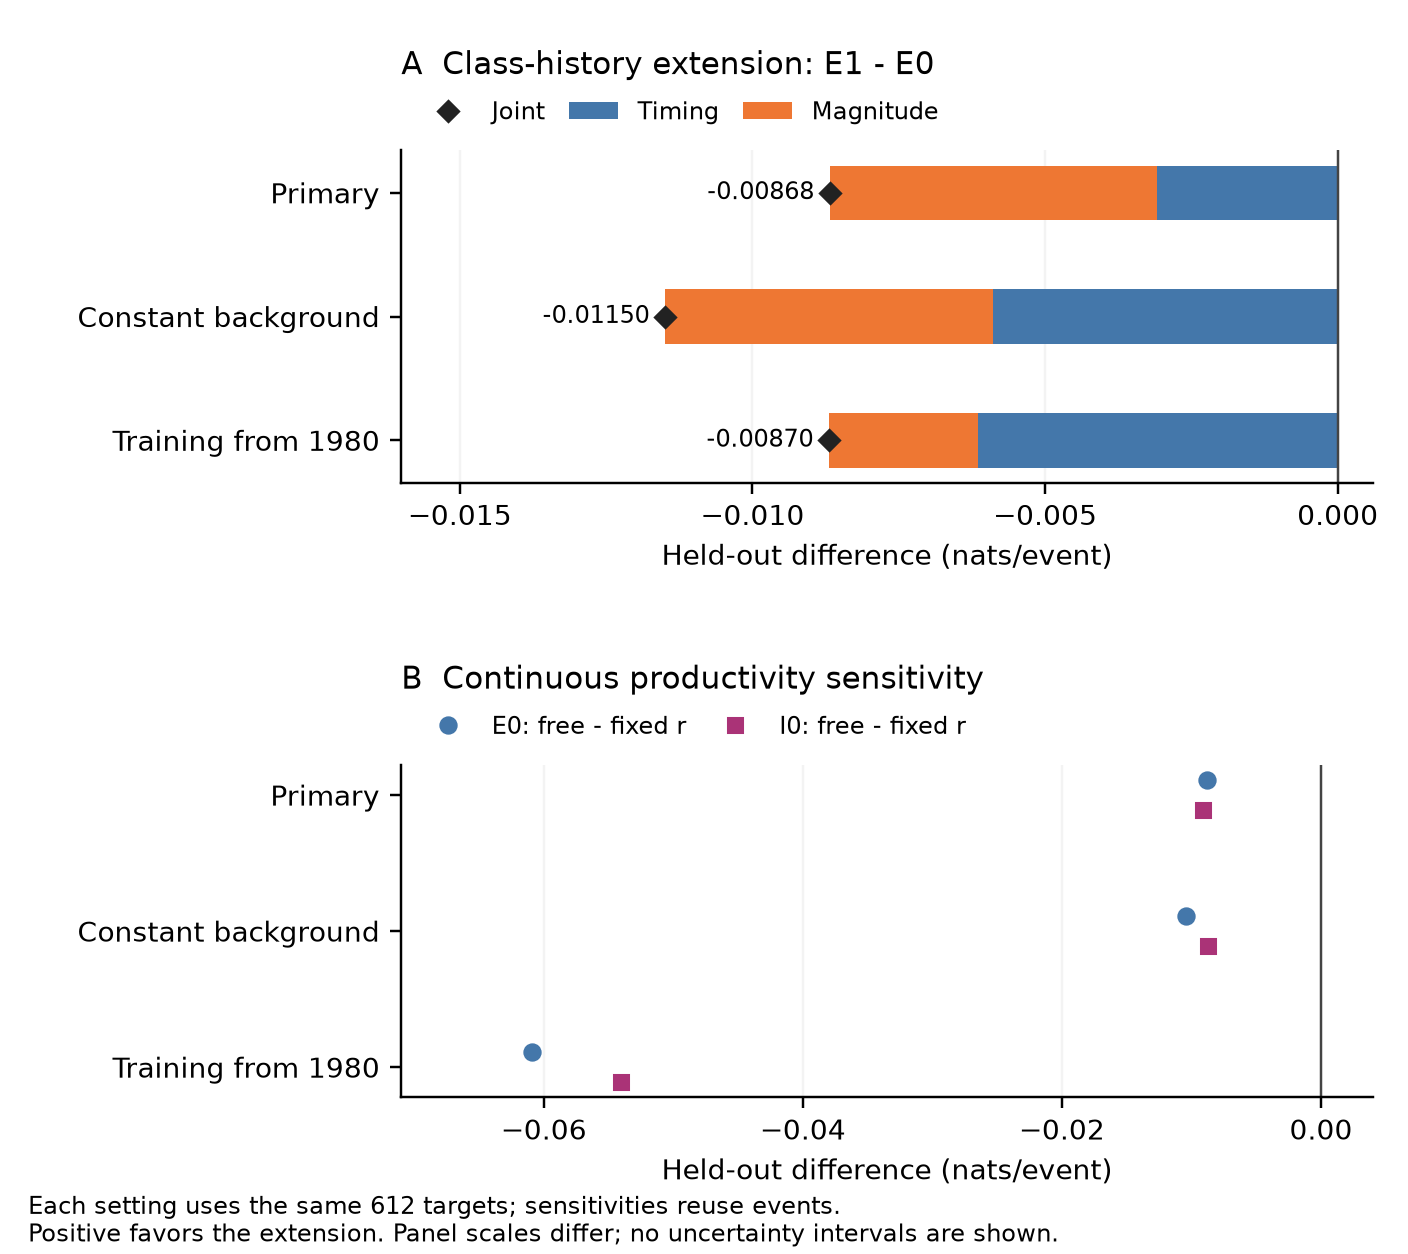
\includegraphics[width=\linewidth]{a2_forecast_comparisons.png}
\caption{Saved aggregate forecast differences. Panel A decomposes the
class-history contrast into timing and magnitude terms; diamonds show their
joint difference. Panel B compares free with fixed productivity in each
ground family. Positive values favor the extension. Each setting reuses
the same 612 targets, the panel scales differ, and no uncertainty intervals
are claimed. Source values are the accompanying reconciled gain tables.}
\label{a2:forecast-figure}
\end{figure}

\section{Interpretation, limitations and disposition}
\label{a2:limits}

The original manuscript, the F nuisance companion and the present
follow-ups address related but distinct questions. The original observed
recipe selected \(r=0.4\) at its first origin and \(r=0.7\) later, with a
different training magnitude-rate estimator. The new comparisons fix
\(r=0.7\) in their reference fits and use a shared training-only
conditional-within-bin estimator. Their matched contrasts are valid
within those separately frozen protocols; they are not corrected entries
in the original paper's predictive table (Chapter~\ref{ch:observed}; Appendix~\ref{app:custody}).

The F checkpoint had 1,528 unknown method outcomes out of 8,596
planned before Stage~2 recovery. Historical counts and accounting bounds
retain their original scope. Neither observed follow-up supplies those
missing null-query results, establishes empirical null size or upgrades a
power comparison. No F fit, bank, calibration or resampling plan was
reopened in this study (Section~\ref{sec:f-continuation}; Appendix~\ref{app:custody}).

The class-history construction is deliberately restricted. The consulted
MDFHP preprint permits class-specific temporal and magnitude-productivity
parameters and bounded class mark distributions, with upper magnitude
10 \citep[Section~2]{DavisBaeumerWangPreprint2024}. Our common-kernel,
low-dimensional \(P(h)\) and source-fertility
contrast, together with an unbounded excess-exponential working law, are
different modelling choices. The conditional summed-intensity identity
depends on those choices. It does not refute the broader class-history
framework, reproduce the authors' Japan or Middle America fits, or
transfer identification and stationarity theorems to a nonlinear
inhibitory family.

All forecast windows had been inspected in earlier research. Training
prefixes overlap and the sensitivity settings reuse the same 612
targets. The results are retrospective exploratory procedure comparisons,
not prospective confirmation or independent replications. Three windows
do not support treating clustered events as independent draws for
standard errors or significance claims. Native magnitude rounding,
mixed magnitude conventions, time-varying detection, missing smaller or
deeper parents, pre-1960 activity and national spatial pooling remain
observation/model assumptions. They were not resolved by these
extensions.

The engineering controls and complete numerical audits make the
implementation inspectable, but do not establish global optima, precise
identification, confidence coverage or power. Positive control examples
show that the fitted pipeline can return gains on particular generating
histories. Equal Perron branching radius did not equate immigrant-weighted
offspring production in the class-active control; different offspring
composition and event counts limit any information-matched comparison.
Sparse profiles and near-training-equivalent candidate spreads retain
their descriptive meanings.

The negative forecast results do not establish that physical inhibition
is absent. Nor do lower fitted slopes establish that \(r=0.7\) is
physically wrong, or show that the earlier negative fertility contrasts
were caused by that fixed value. The cross-run pattern motivates a
possible compensation interpretation, while joint estimation of the
fertility/association extension with free \(r\) remains unperformed.
The persistence of \(E0\)'s forecast advantage over \(I0\) is specific
to the tested recipes and windows.

Both investigations are therefore retained at their respective negative
checkpoints. The fixed-\(r\) \(E0\) candidate remains the predictive
reference for these follow-up comparisons. Broken-slope, saturation,
spatial-locality and independent-data extensions were outside their
executed scope. A future study would require a separately justified
question, information set and protocol, rather than further tuning of
these already examined forecast windows.

\section{Evidence and reproducibility scope}
\label{a2:repro-scope}

The companion records exact protocol, source, score-table and review
identities. The deterministic editorial reconciliation recomputes display
contrasts and counts from saved aggregate/model records using an explicit
hash-bound input list. It does not regenerate scientific histories,
refit models, recalibrate tests or repeat the raw-catalogue auditors.

The original history audit and the later source-reconstructed productivity
audit have different recorded scopes. The latter evaluated all saved
candidates using independently reconstructed geometry rather than merely
checking cache hashes and scoring from production arrays. Their passed
receipts are evidence about the executed checks, not certification of
every mathematical or scientific assertion.

The first API harness and first fresh-control saved-auditor interface
failures in the productivity study remain preserved with their repairs.
The successful append-only auditor corrected terminal-record model-name
extraction without changing scientific fits or tolerances. No control
history was redrawn and no observed outcome refitted in that repair.
A cosmetic profile-figure correction changed marker visibility only.
Earlier engineering adjustments in the history study likewise remain
in its own execution evidence.

The public companion contains the reviewed source and derived score and
parameter display packet, source/result identities and accepted figures.
The exact public manifest identifies its membership. Raw observed catalogue rows and
geometry caches, external article PDFs, private literature inputs and
provider conversations are excluded. Complete raw-geometry replay
requires the separately held matching input and cache files; frozen
absolute paths require an explicit reviewed relocation mapping.
Availability of a compact saved-result packet does not imply availability
of every historical dependency.
The accompanying historical-execution excerpt retains mandatory-start
completion slots and the relevant saved auditor counts and geometry-check
flags, with selectors and original source hashes. It reports prior checks;
no raw-source reconstruction was repeated for this addendum. A separate
boundary inventory distinguishes prescribed coordinates from estimated
constraint hits.

Likelihood and analytic-gradient evaluation run in C++; Python handles
geometry, optimization orchestration, artifact analysis and audits.
MATLAB was unnecessary for these two predictive follow-ups. An earlier
reference-kernel bridge and inspected upstream source are attributed
separately from the independently implemented repeated likelihood.
Existing contributor and AI-assistance disclosures are retained;
computational-agent review is distinct from independent external
human peer review.



\subsection{Data, source and software attribution}

The GeoNet catalogue DOI identifies a continuously updated data resource;
the analyses use the frozen archived selection, whose processed SHA-256 is
\begin{center}\small
\nolinkurl{feacccb7581d1c4c33f88874cd6b198c41639da6930a7fc35e46f910a594fb3e}.
\end{center}
We acknowledge GeoNet and its programme sponsors for the data underlying
the studies. Native magnitude scales and the original selected values are
retained. Neither source citations nor matching archive hashes validate
homogeneity or catalogue completeness.

The Otago implementation was inspected at the separately identified
\emph{MDFHPCode} source commit \citep{MDFHPCode}. An earlier feasibility
reference-kernel bridge is distinct from the independently implemented
finite-mixture objective used in the two predictive follow-ups. Its source
context includes Garrappa's numerical Mittag-Leffler work
\citep{Garrappa2015}. We do not redistribute the upstream general contour
implementation, reference-paper PDFs, upstream binaries or private
literature packet. Citation of a paper and compliance with a code file's
licence are separate responsibilities; no claim of a full MATLAB optimizer
reproduction follows from the reference check.

The recorded pilot environment used Python 3.13.4, NumPy 2.2.6 and SciPy
1.15.3. NumPy, SciPy and Matplotlib are credited for their actual array,
optimization and display roles \citep{Harris2020,Virtanen2020,Hunter2007}.
Repeated likelihood and analytic-gradient work was compiled C++; changing
the compiler or rebuilding a library creates a new binary identity. The
editorial build uses Tectonic 0.17.0, and its source, tool and figure hashes
are recorded separately from the scientific execution records. Font and
package resources were not snapshotted as a byte-identical historical
environment.

\subsection{Versioned evidence and saved-display replay}

The history record is
\nolinkurl{magnitude_prediction_20261023T222049Z}, at checkpoint
\nolinkurl{stop_no_robust_joint_gain}. The productivity record is
\nolinkurl{productivity_slope_20261024T023501Z}, at checkpoint
\nolinkurl{stop_no_robust_productivity_gain}. These local records are
identified by their saved protocol, source and output hashes. The companion
data provide complete case/model score and parameter tables, the saved-count
derivation for the 164 earlier selected parents, and the aggregate values
and cell provenance used here; no
journal DOI or already-published remote record is invented for either run.

Portable display replay reads only the supplied aggregate JSON/CSV packet
and writes to new output directories. It can recreate the gain tables and
figures without fitting models, generating histories or accessing event
rows. The source/replay guide explains commands and omitted dependencies.
The annotated \texttt{scientific\_settings.json} excerpt retains the
kernel/stress constants, solver and profile policies, and continuation
gates, with the original producer-protocol hashes. It is not a replacement
frozen protocol. For the Mittag-Leffler representation, the serialized
\(p=1.3\) field is inactive rather than an additional fitted kernel shape.
This is different from repeating the original raw-data auditors or
reconstructing every historical scientific source epoch. Original
absolute-path producer records retain their old identities; a relocated
raw-data replay needs an explicit reviewed mapping and matching private
inputs.

\begin{figure}[p]
\centering
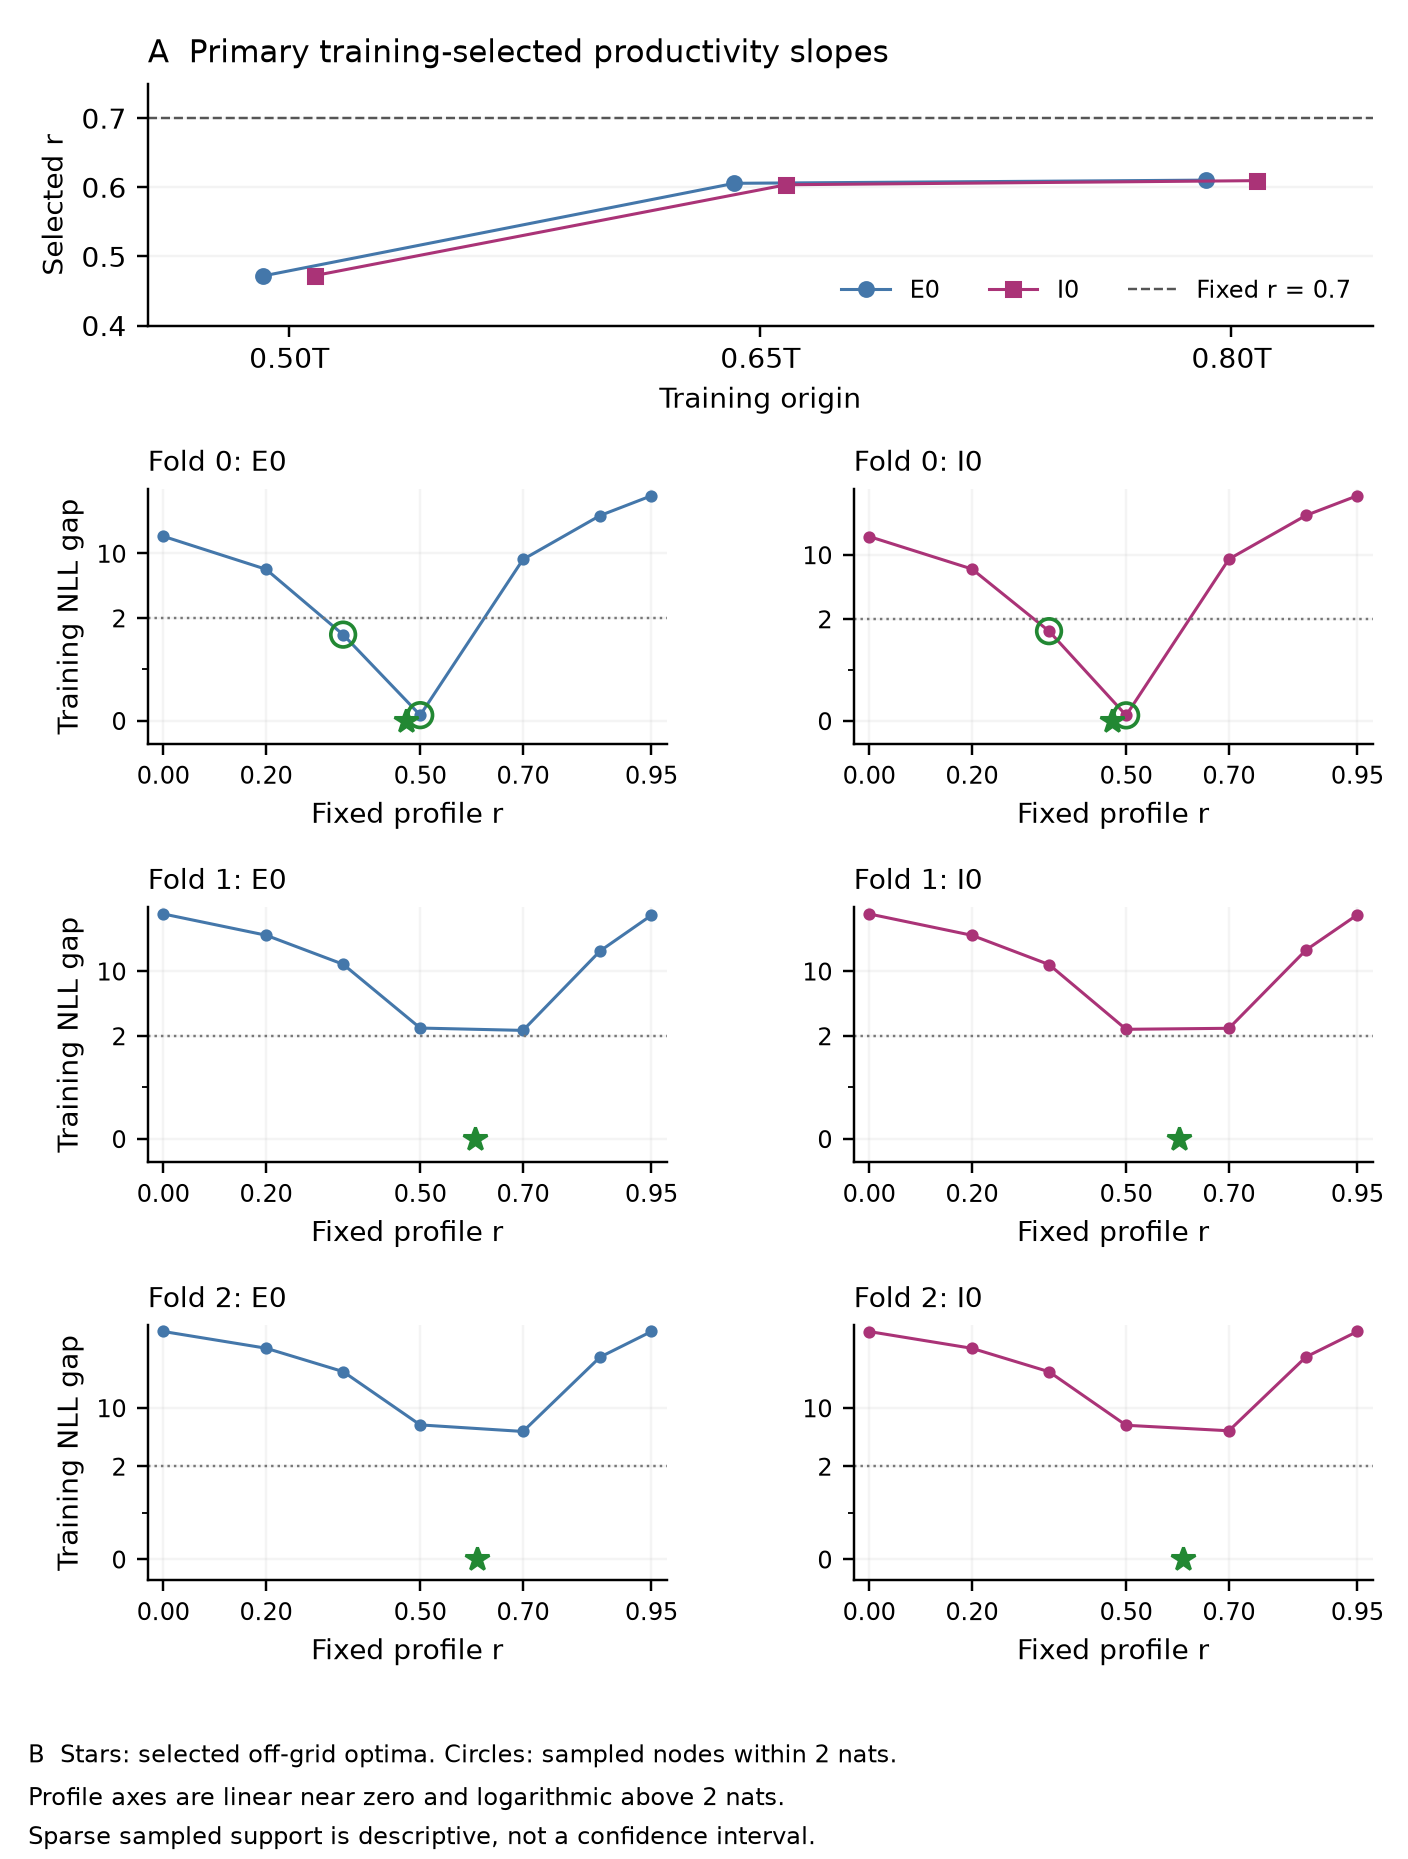
\includegraphics[width=\linewidth,height=.78\textheight,keepaspectratio]{a2_productivity_profiles.png}
\caption{Primary training-selected productivity ratios and the seven-node
descriptive profiles. Stars show selected off-grid optima; circles identify
sampled points within two nats. The profile vertical axes are linear near
zero and logarithmic above two nats. Empty sampled support in four panels
does not define an empty confidence interval. All values are saved training
results; profile forecasts did not select parameters.}
\label{a2:profile-figure}
\end{figure}

\noindent The complete magnitude-extension fold accounting is retained in \hyperref[app:audit09-magnitude-folds]{Appendix~\ref{app:audit09-magnitude-folds}}.

\section{Exposure orthogonalization and the Stage A coarse-kernel comparison}
\label{sec:stage-a}
Let $w_l>0$ be the normalized training exposure quadrature weights and write
$\bar x=\sum_lw_lx_{\mathrm{trend}}(t_l)$, $\bar G=\sum_lw_lG_l$. Provided
$V_x=\sum_lw_l(x_{\mathrm{trend}}(t_l)-\bar x)^2>0$, define
\[
 \gamma_1=\frac{\sum_lw_l(x_{\mathrm{trend}}(t_l)-\bar x)(G_l-\bar G)}{V_x},\qquad
 \gamma_0=\bar G-\gamma_1\bar x,\qquad R=G-\gamma_0-\gamma_1x_{\mathrm{trend}}.
\]
Then $\sum_lw_lR_l=\sum_lw_lx_{\mathrm{trend}}(t_l)R_l=0$ algebraically. The coefficients
are estimated from training exposure only and frozen for prediction and
order-32 checking. Refitting them on the verification grid would change the
model. Degenerate exposure variance invalidates the two-coordinate projection;
zero residual variance reports redundancy rather than identification.
The unrestricted map is exact:
\[
 \widetilde a=a-\eta\gamma_0,\quad
 \widetilde d=d-\eta\gamma_1,\qquad
 a=\widetilde a+\eta\gamma_0,\quad
 d=\widetilde d+\eta\gamma_1.
\]
Thus $a+dx_{\mathrm{trend}}-\eta G=\widetilde a+\widetilde d x_{\mathrm{trend}}-\eta R$ at every time.
Equal numerical boxes in these coordinates describe different constrained
families; mapped floors are admissible only when all destination restrictions
hold, without clipping. An $\eta$-only ridge is invariant under this map.
Raw $d=0$ differs from residual $\widetilde d=0$. The residual can be negative,
so the detrended background may locally exceed its nominal undepleted level.
Exposure orthogonality is not likelihood-score orthogonality: event scores
contain $B/\lambda$, information involves $B^2/\lambda$, and projection onto
$(1,x_{\mathrm{trend}})$ does not remove dependence on the excitation-amplitude score.

For $B=\exp(\widetilde a+\widetilde d x_{\mathrm{trend}}-\eta R)$ and
$\lambda=B+nH$, let $J$ be complete productivity-weighted trigger exposure.
The timing negative log likelihood and gradient are
\begin{align*}
 L&=\sum_lq_lB_l+nJ-\sum_i\log\lambda_i,\\
 L_{\widetilde a}&=\sum_lq_lB_l-\sum_i B_i/\lambda_i,&
 L_{\widetilde d}&=\sum_lq_lx_{\mathrm{trend}}(t_l)B_l-\sum_i x_{\mathrm{trend}}(T_i)B_i/\lambda_i,\\
 L_n&=J-\sum_iH_i/\lambda_i,&
 L_\eta&=-\sum_lq_lR_lB_l+\sum_iR_iB_i/\lambda_i.
\end{align*}
The raw formulas replace $R$ by $G$. At $n=0$, $L_n$ remains well defined;
at $\eta=0$, values and shared-coordinate gradients must nest using a common
integration branch or an explicitly controlled numerical seam.

Stage A selected Omori triggering by training excitation-only fits on the
nine-point grid $c\in\{0.1,1,10\}$ days and $p\in\{1.1,1.3,1.7\}$.
The selected kernel was frozen for its excitation/inhibition pair. The stress
survival law and $r=0.7$ remained fixed. This is a restricted coarse-grid
procedure, distinct from the historical continuously refined Omori fit and
the later continuous Extension O.
\section{Stage A saved evidence and interpretation}


All planned procedures are complete and independently audited. A negative predictive result is a completed Stage A result.

\subsection{Aggregate held-out comparisons}


The variants reuse the same targets. Mark-score differences cancel; timing is the event plus compensator contribution. In primary, exposure orthogonalization changes the pooled ML inhibition contrast by only \(-0.000045575\) nats, from \(-18.186415\) to \(-18.186460\) nats. The raw interior optimum maps feasibly into the orthogonal box; better Gram conditioning therefore does not change the represented optimum materially.





\subsection{Interpretation limits}


Orthogonalization is an invertible unrestricted coordinate transformation. Identical boxes in raw and transformed coordinates define different constrained families, including intercept constraints. The projection removes exposure drift; it does not establish likelihood-score orthogonality. Constant-background restrictions have different meanings in the two coordinates.

Omori parameters were selected by training E0 on the fixed nine-point grid and shared within each excitation/inhibition pair. The ML stress survival law and r=.7 remained fixed. This is not exact replication of Iteration27 continuous kernel/productivity selection.

Historical Fold0 raw inhibition loss around -16.99 nats is contextual. Compare against the newly recomputed raw baseline and retain differences due to nuisance/optimizer estimation. Selected parameters, mapped feasibility, bound flags, training-only coefficients and Gram diagnostics are saved in results/analysis.

Previously inspected chronological windows and one regional catalogue support descriptive predictive comparisons only. No event-iid confidence intervals, Wilks boundary claims, global-optimum certificate or physical-causality assertion. Stage A preceded the completed Stage B and C studies reported later in this volume.

\subsection{Audit}


The independent auditor reconstructed local raw rows, nuisance estimates, kernels, quadrature and projection; checked every saved candidate and solver return, exact floors, all planned start slots and aggregate score entries. Internal optimizer line-search iterates were not all serialized.

\subsection{Fold0 reconciliation}


Historical rawI-minus-E0: -16.988778741 nats; recomputed rawI-minus-E0: -16.988735123; difference: +0.000043618.
Orthogonal ML inhibition minus E0: -16.988768914; orthogonal-minus-raw improvement: -0.000033791 nats.
Matched Omori inhibition minus its E0: -16.404033164; Omori E0 minus ML E0: -3.210666185; combined orthogonal Omori minus ML E0: -19.614699350 nats.
These are arithmetic contrasts of separately trained constrained procedures, not a causal decomposition.




\noindent The stage A complete fold score accounting is retained in \hyperref[app:audit09-stage-a-folds]{Appendix~\ref{app:audit09-stage-a-folds}}.

\subsection{Stage A complete aggregate score accounting}
Comparison keys are local to this table. 
\begin{description}
\item[AG1] \path{I0_raw_ml-E0_ml}
\item[AG2] \path{I0_orth_ml-E0_ml}
\item[AG3] \path{I0_orth_ml-I0_raw_ml}
\item[AG4] \path{E0_omori-E0_ml}
\item[AG5] \path{I0_orth_omori-E0_omori}
\item[AG6] \path{I0_orth_omori-I0_orth_ml}
\item[AG7] \path{(I0_orth_omori-E0_omori)-(I0_orth_ml-E0_ml)}
\end{description}

\noindent The stage A aggregate sensitivity accounting is retained in \hyperref[app:audit09-stage-a-sensitivity]{Appendix~\ref{app:audit09-stage-a-sensitivity}}.

{\small
\setlength{\tabcolsep}{3pt}
\begin{longtable}{lrrrrrr}
\caption{Stage A complete aggregate score accounting; primary. Total nats unless stated otherwise. Positive favors the candidate. The same 612 targets enter each aggregate; positive-fold counts are out of three.}\label{tab:AG-primary}\\
\toprule
Key & $\Delta Q$ & $\Delta C$ & Timing & $\Delta M$ & Joint & Joint/event\\\midrule
\endfirsthead
\toprule
Key & $\Delta Q$ & $\Delta C$ & Timing & $\Delta M$ & Joint & Joint/event\\\midrule
\endhead
AG1 & -40.854975 & 22.668560 & -18.186415 & 0.000000 & -18.186415 & -0.029716\\
AG2 & -40.855042 & 22.668582 & -18.186460 & 0.000000 & -18.186460 & -0.029716\\
AG3 & -0.000068 & 0.000022 & -0.000046 & 0.000000 & -0.000046 & -0.000000\\
AG4 & -38.017200 & -0.154092 & -38.171292 & 0.000000 & -38.171292 & -0.062371\\
AG5 & -36.772664 & 20.496091 & -16.276573 & 0.000000 & -16.276573 & -0.026596\\
AG6 & -33.934822 & -2.326583 & -36.261405 & 0.000000 & -36.261405 & -0.059251\\
AG7 & 4.082379 & -2.172491 & 1.909887 & 0.000000 & 1.909887 & 0.003121\\
\bottomrule
\end{longtable}
}

\noindent The stage A training exposure geometry is retained in \hyperref[app:audit09-stage-a-geometry]{Appendix~\ref{app:audit09-stage-a-geometry}}.

\section{Stage B: common and parent-class temporal scales}
\label{sec:stage-b}
For a pinned positive mixture with $\sum_mw_m=1$, use $s=\log\tau$ and
$a_m=\lambda_m e^{-s}$ to write
\[
 k_s(u)=\sum_mw_ma_me^{-a_mu},\qquad S_s(u)=\sum_mw_me^{-a_mu}.
\]
Every scale preserves unit mass; the parent's observed class selects its
entire kernel. The prospective range was $\tau\in[0.001,20]$ days,
including subhour scales. This is no cutoff on the retained parent history.
At $y=a_mu$,
\[
 \partial_s k_s(u)=\sum_mw_ma_me^{-y}(y-1).
\]
For a parent's finite-window lag interval $[L,U]$,
\begin{align*}
 J_k(s)&=\sum_mw_me^{-a_mL}\{-\operatorname{expm1}[-a_m(U-L)]\},\\
 \partial_sJ_k&=\sum_mw_m\{a_mLe^{-a_mL}-a_mUe^{-a_mU}\}.
\end{align*}
Productivity weights multiply these expressions; all earlier parents and quiet
exposure remain. Lags, rather than edited cached kernel values, define dynamic
evaluation. The fixed-scale, common-free and class-free models respectively
fix both scales to one day, estimate a common scale, and estimate two parent
scales. All use $h=\delta=0$, fixed $r=0.7$ and the common training magnitude
law. The common gradient is the sum of class gradients on the diagonal;
at $n=0$ all scale derivatives vanish and the scales are unidentified.

The optional association family preserves the original Perron normalization:
\[
 \lambda_i=p_iB+\frac n{\rho(h)}\sum_jP_{ij}(h)H_j,\qquad
 \Lambda=B+\frac n{\rho(h)}(H_0+H_1).
\]
Unit temporal mass makes $\rho$ independent of the scales. Column stochasticity
still cancels target redistribution even with different parent kernels.
At fixed effective amplitude $n/\rho(h)$, timing is invariant to $h$ wherever
the map remains feasible; conditional marks can change. Joint refitting and
box constraints may indirectly change timing. No target-class temporal family
was introduced to evade this identity.

For $\Gamma=n/\rho$, $T_i=\sum_jP_{ij}H_j$ and
$e_i=p_iB+\Gamma T_i$, the optional joint negative log likelihood is
\[
 L=\int B+\Gamma(J_0+J_1)-\sum_i\log e_i
   -\sum_i\{\log f_\beta(q_i)-\log p_i\}.
\]
Its scale gradient is
$L_{s_j}=\Gamma J'_j-\sum_i\Gamma P_{ij}H'_j/e_i$ and
\[
 L_h=-\Gamma\frac{\rho'}\rho(J_0+J_1)
 -\sum_i\frac{\Gamma\{\sum_jP'_{ij}H_j-(\rho'/\rho)T_i\}}{e_i},
 \quad P'_{ij}=\mathbf1_{i=j}-p_i.
\]
The nuisance $\beta,p_i$ are training-frozen. At $n=0$, association and scale
gradients vanish. All prescribed starts and exact nested floors must resolve;
a finite candidate cannot replace an incomplete start. Near-training-equivalent
candidates within $4\times10^{-4}$ NLL receive full forecast checks with spread
strictly below $0.01$ nats/event.
\section{Stage B audited results, historical bridge and failed association gate}


Allowing one common Mittag-Leffler timescale improves pooled event-timing forecasts in all three retained windows. Additional parent-class timescales give a small positive aggregate gain, but improve only one window against the common-scale model. The predeclared association gate therefore fails, and no observed h model was fitted. This is a completed gated investigation, not a negative result for the unexecuted h branch.

\subsection{Audited comparisons}


All nine observed fit procedures and 72 prescribed starts completed. The independent raw-row audit reconciled 90 candidates and 72 solver returns, with no failed finite solver returns. The two fixed-seed engineering histories also completed eight procedures/64 starts, including the optional h engine. Near-optimal forecast stability and source/input integrity gates passed.

The 612 targets occur in disjoint chronological windows containing 203, 155 and 254 events; their training prefixes overlap. All three observed models use fixed r=0.7, the same training-only beta per case, h=0 and the same magnitude density. Mark differences cancel up to floating-point roundoff, so timing and joint gains coincide.


Here the historical E field is the ground event-log-intensity contrast, denoted $\Delta Q$ in this volume and C is the baseline-minus-candidate compensator, so $\Delta Q+\Delta C$ equals timing. Timing plus the conditional-mark contrast equals joint score. These are event-weighted sums divided by 612, rather than unweighted averages of fold rates.


The common-scale gain is consistent across these windows, although Fold 0's gain is only 0.077011 nats. The class-specific aggregate is positive, not a net loss. Its inconsistency against the stronger common-scale comparator is the reason the next branch stops. Winning two windows against the fixed tau=1 baseline is not the declared gate.

\subsection{Scale and selection limits}


All selected parameters are interior to their prescribed bounds. The allowed tau range was 0.001 to 20 days, including subhour values, but none of the observed fitted scales is subhour. There is no lower-bound truncation explanation for these selected estimates and no bound expansion was performed.

Class 0 means 5.0$\leq$M<5.5 and class 1 means M$\geq$5.5. The kernels attach to the parent's class. The fitted ordering changes: class 0 is faster in Fold 0 but slower in Folds 1 and 2. These fits do not establish a stable physical magnitude ordering of aftershock timescales. Tau is a normalized-kernel scale, not a finite aftershock-duration cutoff, and is not interchangeable with Omori c.

Training NLL improves under exact nested floors. The additional class-specific training gains against the common model are approximately 0.012055, 1.867655 and 5.248592 nats, yet two held-out windows lose. Neither training improvement nor passing near-optimal forecast checks certifies physical scale identification or a global optimizer.

\subsection{Optional association branch}


The prospective rule required class-specific h=0 timing to exceed common-scale timing by more than 0.0001 total nats in at least two windows, after complete fitting, independent audit and forecast stability. Only Fold 1 qualifies. The audited gate is false: zero of the conditional three observed h procedures/24 starts were executed. The h code, derivatives and synthetic engineering were validated before observing this decision; engineering validation is not observed evidence for or against association.

The optional mathematical family preserves the legacy Perron normalization. With parent-class kernels, summing the column-stochastic transition matrix still gives ground intensity B+(n/rho(h))(H0+H1). Association h adds no new direct temporal shape conditional on observed parent history; its scalar n/rho effect is already an excitation-amplitude coordinate. At fixed effective amplitude, timing is invariant to h, while conditional mark probabilities can change. No target-class kernels or post-gate model family were introduced.

\subsection{Historical Omori reference}


The immutable historical Omori total is -990.170063 joint nats. The new fixed-scale, common-scale and class-scale procedures have raw joint totals of approximately -984.684158, -977.300484 and -976.292651. Their raw differences from historical Omori are +5.485905, +12.869579 and +13.877412 nats, respectively.

These are descriptive cross-procedure comparisons, not matched kernel-only gains. Historical selected productivity ratios are [0.4,0.7,0.7], whereas B fixes 0.7 throughout; only Fold 0 has that productivity mismatch. All three historical beta estimates use a different global-MLE convention. Beta also enters productivity weights, so this difference affects timing as well as magnitude scores. Historical Omori also used its own continuous shape/scale selection.

For common free tau, the raw historical difference splits into +10.389214 timing and +2.480366 magnitude nats. Magnitude terms therefore cannot be cancelled across those recipes. The matched B free-scale gain remains +7.383674 nats; the larger historical difference cannot be attributed solely to freeing tau. No prior Omori fit was rerun or overwritten, and no new matched Omori model was fitted.

\subsection{Delimited conclusion}


The supported result is a modest, consistent timing gain from a common free ML scale in this bounded pooled procedure. Parent-class scales add a smaller positive aggregate but fail the predeclared across-window continuation criterion. Optional h remains untested on observed data.

This retains the original regional B design despite earlier spatial results; it is not a combined spatial-temporal validation or an independently replicated catalogue. All windows were previously examined. No physical causality, event-iid confidence interval, Wilks boundary inference, global-optimum certificate, alternative bounds or automatic further study is warranted.


\noindent The stage B complete fold score accounting is retained in \hyperref[app:audit09-stage-b-folds]{Appendix~\ref{app:audit09-stage-b-folds}}.

\subsection{Stage B complete aggregate score accounting}
Comparison keys are local to this table. 
\begin{description}
\item[BG1] \path{E0_tau_free-E0_tau1}
\item[BG2] \path{E1_tau_class-E0_tau_free}
\item[BG3] \path{E1_tau_class-E0_tau1}
\end{description}

{\small
\setlength{\tabcolsep}{3pt}
\begin{longtable}{lrrrrrrr}
\caption{Stage B complete aggregate score accounting; primary. Total nats unless stated otherwise. Positive favors the candidate. The same 612 targets enter each aggregate; positive-fold counts are out of three.}\label{tab:BG-primary}\\
\toprule
Key & $\Delta Q$ & $\Delta C$ & Timing & $\Delta M$ & Joint & Joint/event & Positive folds\\\midrule
\endfirsthead
\toprule
Key & $\Delta Q$ & $\Delta C$ & Timing & $\Delta M$ & Joint & Joint/event & Positive folds\\\midrule
\endhead
BG1 & 4.405481 & 2.978194 & 7.383674 & 0.000000 & 7.383674 & 0.012065 & 3\\
BG2 & 5.297977 & -4.290144 & 1.007833 & 0.000000 & 1.007833 & 0.001647 & 1\\
BG3 & 9.703458 & -1.311951 & 8.391507 & 0.000000 & 8.391507 & 0.013712 & 2\\
\bottomrule
\end{longtable}
}

\noindent The stage B selected temporal scales are retained in \hyperref[app:audit09-stage-b-scales]{Appendix~\ref{app:audit09-stage-b-scales}}.

\section{Extension O: continuously tuned, kernel-matched inhibition}

The Omori--Utsu temporal law is a standard aftershock-decay model \citep{Utsu1995}; the comparisons below concern its declared fitted implementation and bounds.
\label{sec:extension-o}
For $u\geq0$, use the normalized Omori density and survival
\[
 k(u)=\frac{p-1}{c}(1+u/c)^{-p},\quad
 S(u)=(1+u/c)^{1-p},\qquad c>0,\ p>1.
\]
With $s=\log c$, $A(u)=\log(1+u/c)$ and $v=u/(c+u)$,
\[
 \partial_s\log k=-1+pv,\quad
 \partial_p\log k=(p-1)^{-1}-A,\quad
 \partial_sS=(p-1)vS,\quad \partial_pS=-AS.
\]
Parent exposure is $J=S(L)-S(U)$ and its derivatives use the same endpoint
differences; stable evaluation uses $S(L)\{-\operatorname{expm1}[(1-p)
(A(U)-A(L))]\}$. No lag truncation is used. The prospectively fixed bounds
are $c\in[10^{-4},20]$ days and $p\in[1.01,2.5]$. These numerical domains
do not identify physical duration or justify an outcome-dependent expansion.
For $z\in\{s,p\}$ the additional timing gradient is
\[
 L_z=n\sum_k\kappa_k\partial_zJ_k
          -\sum_i\frac{n\partial_zH_i}{\lambda_i}.
\]
The stress feature remains the original unit-scale ML survival history and
has no $c,p$ derivative. Both kernel gradients vanish at $n=0$.

The primary excitation fit selects $(c,p)$ by training NLL and shares those
values exactly with raw and orthogonal matched inhibition. The jointly tuned
orthogonal inhibitory fit is secondary. Exact Poisson/nested floors and the
sealed coarse Stage A excitation point are reevaluated in the new objective;
old scores are neither overwritten nor substituted. Every procedure uses its
prescribed starts, with training-only selection and the saved forecast-stability
gate. The same coordinate map and feasibility requirements from Stage A apply.

For the raw inhibited engineering law, the valid thinning envelope is the
undepleted background plus excitation; current inhibited intensity is not a
monotone envelope because stress may recover between events. Independent time
and mark streams, rejection records, caps and unreplaced failed histories are
part of engineering eligibility. A matched training-selected kernel need not
equal the generating kernel; no invalid truth-containment claim follows.
\section{Extension O audited results and sensitivity interpretation}


Continuously training-tuned Omori excitation improved held-out timing over the fixed ML baseline in all three primary windows. Stress inhibition still reduced aggregate held-out scores under the same E-selected Omori kernels. The primary matched orthogonal contrast lost 14.137174 nats across 612 targets, and the secondary jointly tuned inhibitory model lost 11.803237 nats. This is a negative result for the implemented bounded stress-depletion procedures, alongside a positive result for temporal-kernel tuning.

All 45 planned procedures and 360 prescribed starts completed; the independent raw-row audit reconciled 456 candidates and 360 solver returns and found stable near-optimal forecasts. Model selection used training NLL only. Magnitude scores are identical within each case, so every displayed timing difference is also the joint difference.


The matched orthogonal model won only Fold 1 by 0.175158 nats and lost Folds 0 and 2. The jointly tuned inhibitory model lost all three primary windows. Its 2.333937-nat aggregate improvement over matched orthogonal inhibition is secondary; it does not turn the inhibitory versus excitatory comparison positive.

For E\_omori minus E\_ml, the event-log-intensity gain was 17.242145 nats and the compensator contribution was -5.036642 nats, giving +12.205503. For matched orthogonal inhibition minus E\_omori, the event contribution was -37.002313 and the compensator contribution +22.865140, leaving -14.137174. Lower exposure could not offset lost event intensity.

The training-selected primary excitation kernels are reported in Table~\ref{tab:o-kernels} in Appendix~\ref{app:audit09-extension-o-kernels}.


These c and p estimates are interior to the prospectively fixed bounds. The short selected c values explain why the earlier coarse grid with minimum c=0.1 day did not adequately search this continuous family. This is a scale parameter of a heavy-tailed kernel, not an estimated physical recovery duration. Stress itself still uses the original fixed ML survival kernel; only triggering was continuously tuned.

Orthogonalization did not rescue the primary loss. In Fold 0 raw inhibition reached its raw d=2 upper boundary. Its selected point maps feasibly into orthogonal coordinates, while the orthogonal optimum maps back to raw d=2.114439 and lies outside the raw box. The orthogonal fit improves training NLL by only 0.005858 nats but loses a further 0.361471 test nats. In Folds 1 and 2 the selected points map feasibly both ways and their forecasts agree up to numerical optimization differences. Thus the small primary difference between raw and orthogonal procedures is explained by a changed bounded parameter domain, rather than a new unrestricted model space. Exposure orthogonality is not likelihood-score orthogonality.

The constant-background sensitivity fixes raw d=0 or detrended d\_tilde=0 respectively. These are different restrictions; all selected mapped raw/orth constant-case points violate the destination constant restriction. Their contrast cannot be interpreted as pure reparameterization. The post-1980 variant changes the training window and its projection/nuisance estimates, while retaining full prior event history.


Omori excitation wins all three windows in each sensitivity variant. Every inhibitory aggregate remains negative. Constant-background detrended inhibition improves over raw inhibition by 5.449474 nats, but still loses 8.796918 nats against its matched excitatory comparator. The same test events are reused across variants and must not be pooled as 1,836 independent targets.

Within this bounded, regionally pooled fixed-productivity family, inhibitory failure therefore persists after replacing the inferior fixed ML trigger with continuously tuned Omori excitation. It cannot be attributed solely to that fixed-trigger choice or solely to the raw trend boundary. This does not establish that physical stress inhibition is absent, and it does not test continuous spatial stress or a joint spatial/temporal extension. The historical Iteration 27 Omori result uses a different nuisance recipe, including the Fold 0 productivity ratio and training magnitude estimator; the present gain is a new internally matched comparison, not a numerical reproduction of that historical score.

The catalogue and windows were previously inspected, and three chronological tests provide limited robustness evidence. No event-iid intervals, boundary Wilks claims, physical-causality conclusions or global-optimum certificate follow. S was designed and frozen before these outcomes; its launch is governed by correctness and resource admission, not this score direction.

Exact per-window scores, parameters, boundary flags and both-direction mapping diagnostics are in summary.json. The independent raw-row reconciliation is in observed\_saved\_audit\_v1.json.

\noindent The extension O complete fold score accounting is retained in \hyperref[app:audit09-extension-o-folds]{Appendix~\ref{app:audit09-extension-o-folds}}.

\subsection{Extension O complete aggregate score accounting}
Comparison keys are local to this table. 
\begin{description}
\item[OG1] \path{E_omori-E_ml}
\item[OG2] \path{Iorth_matched-E_omori}
\item[OG3] \path{Iraw_matched-E_omori}
\item[OG4] \path{Iorth_joint-E_omori}
\item[OG5] \path{Iorth_joint-Iorth_matched}
\item[OG6] \path{Iorth_matched-Iraw_matched}
\end{description}

\noindent The extension O aggregate sensitivity accounting is retained in \hyperref[app:audit09-extension-o-sensitivity]{Appendix~\ref{app:audit09-extension-o-sensitivity}}.

{\small
\setlength{\tabcolsep}{3pt}
\begin{longtable}{lrrrrrrr}
\caption{Extension O complete aggregate score accounting; primary. Total nats unless stated otherwise. Positive favors the candidate. The same 612 targets enter each aggregate; positive-fold counts count joint gains exceeding $10^{-4}$ nats out of three. Positive values at or below that threshold are treated as numerical ties.}\label{tab:OG-primary}\\
\toprule
Key & $\Delta Q$ & $\Delta C$ & Timing & $\Delta M$ & Joint & Joint/event & Positive folds\\\midrule
\endfirsthead
\toprule
Key & $\Delta Q$ & $\Delta C$ & Timing & $\Delta M$ & Joint & Joint/event & Positive folds\\\midrule
\endhead
OG1 & 17.242145 & -5.036642 & 12.205503 & 0.000000 & 12.205503 & 0.019944 & 3\\
OG2 & -37.002313 & 22.865140 & -14.137174 & 0.000000 & -14.137174 & -0.023100 & 1\\
OG3 & -36.491541 & 22.715835 & -13.775706 & 0.000000 & -13.775706 & -0.022509 & 1\\
OG4 & -27.179752 & 15.376515 & -11.803237 & 0.000000 & -11.803237 & -0.019286 & 0\\
OG5 & 9.822562 & -7.488625 & 2.333937 & 0.000000 & 2.333937 & 0.003814 & 1\\
OG6 & -0.510772 & 0.149304 & -0.361468 & 0.000000 & -0.361468 & -0.000591 & 0\\
\bottomrule
\end{longtable}
}

\noindent The extension O selected continuous kernels are retained in \hyperref[app:audit09-extension-o-kernels]{Appendix~\ref{app:audit09-extension-o-kernels}}.

\section{Engineering witnesses and constrained-map diagnostics}
\subsection{Control normalization and saved forecast contrasts}
These are particular fixed engineering realizations. Equal Perron radii do
not equalize immigrant-weighted first-generation production, event counts or
statistical information. In particular the class-active laws can dilute the
offspring contribution. All controls remain visible, including losses, rather
than retaining only successful examples. These tables support implementation
inspection, not calibrated power, bias, coverage or reliable recovery.

\noindent The engineering normalization, forecast, profile and map witnesses are retained in \hyperref[app:audit09-engineering-witnesses]{Appendix~\ref{app:audit09-engineering-witnesses}}.

\subsection{Coarse-grid loss and the later continuous-kernel gain}
The coarse Stage A excitation-only Omori procedure lost to its matched ML
reference in every aggregate setting: primary -38.171292, post-1980 -15.005799 and constant-background -43.433403 nats.
Every excitation-selected scale in Table~\ref{tab:a-coarse-kernels} is at the
lower coarse-grid endpoint, $c=0.1$ day. In contrast, continuous Extension O
gained 12.205503 primary nats over its matched ML reference, with all three windows positive.
This is a materially different outcome from the coarse-grid loss. The continuous
primary selected scales lie below the earlier grid, but these results compare
bounded fitted procedures; they do not identify a universal kernel ranking.

\noindent The stage A selected coarse-grid kernels are retained in \hyperref[app:audit09-coarse-kernels]{Appendix~\ref{app:audit09-coarse-kernels}}.

\subsection{Engineering-clock and evaluation scope}
Stage B's two engineering laws fixed a common scale of $0.02$ day or parent
scales $(0.005,0.5)$ day, with log immigration $a=\log(0.4)$, $d=0$,
$n=0.2$, $\beta=2.85$, $r=0.7$, a $500$-day horizon and training ending at
day $350$. The horizon was fixed before generation to retain expected
immigration while reducing binary64 clock spacing relative to the earlier
$5000$-day engineering design. It did not rescale observed data or change the
absolute scale bounds. In the uninhibited constant-background controls,
inversion of the exact integrated hazard needs no acceptance uniform because
envelope and actual intensity agree. Independent time and mark streams,
retained sampled versus actual binary64 elapsed times and fail-without-jitter
clock rules remain essential. Known synthetic nuisance values and the observed
training-only nuisance adapter have distinct verification roles. The optional
association engine was exercised on both controls before the observed gate;
this supplies no observed evidence about the unexecuted association branch.

The common-scale and parent-scale engineering laws are deliberately fixed
examples, not estimates of a physical ordering. Saved numerical derivatives,
exact nested floors, left limits, complete parent exposure and direct-history
truth checks delimit implementation validity. A repaired control or audit
interface does not authorize replacing failed histories or promoting an
unresolved production outcome. No new engineering computation accompanied
that historical consolidation.

\section{Completed matched magnitude-history experiment}

\label{sec:s02-completed}

\textit{Execution provenance: the original completed campaign passed the saved custody checks and predeclared independent raw sample. Acceptance uses sampled validation, not independent replay of every fit. This edition recovered and verified the original histories, selected fit states and attempt records; it did not rerun the fitting campaign.}

The experiment uses 100 paired forest units and 300 catalogues across persistence settings $h\in\{0,0.5,0.9\}$. The strictly subcritical generator has productivity ratio $r=0$ and reproduction mean $n=0.5$. Each catalogue is fitted by M1, the misspecified $r=0.7$ candidate, and M2, the productivity-matched $r=0$ candidate. Both hold $n=0.5$ and use the same inherited kernels and eight-start null/alternative procedure, fitting the background level, trend and stress coefficient. All 600 procedure--catalogue cases are complete; no seed was redrawn.

M1 is a structural replication arm, not an exact numerical replication of the earlier pilot: the common reproduction mean and strengthened starts are disclosed. M2 matches productivity at $h=0$, but the exact Mittag--Leffler generator and finite 195-mode candidate still differ numerically. It is therefore not described as a literally exact full null law.

\begin{table}[htbp]\centering\setlength{\tabcolsep}{5pt}

\caption{Completed selection counts and descriptive empirical calibration. Selection uses $\mathrm{GLR}>0.001$ and $\hat\eta>10^{-6}$. All entries have 100 resolved catalogues; intervals are 95\% Wilson intervals for selection proportions.}\label{tab:s02-completed}

\begin{tabular}{llrrrr}\toprule

Procedure & $h$ & Selected & Wilson interval & Empirical $h=0$ threshold & Above threshold\\\midrule

M1 & 0.0 & 79/100 & [0.700, 0.858] & 7.665955 & 4/100 \\

M1 & 0.5 & 85/100 & [0.767, 0.907] & 7.665955 & 6/100 \\

M1 & 0.9 & 85/100 & [0.767, 0.907] & 7.665955 & 6/100 \\

M2 & 0.0 & 75/100 & [0.657, 0.825] & 4.629883 & 4/100 \\

M2 & 0.5 & 75/100 & [0.657, 0.825] & 4.629883 & 4/100 \\

M2 & 0.9 & 69/100 & [0.594, 0.772] & 4.629883 & 4/100 \\

\bottomrule\end{tabular}\end{table}

The empirical threshold is the higher empirical 95th percentile of the same 100 $h=0$ GLRs within each procedure. The four strict exceedances among those same controls are a consequence of this in-sample construction and ties, not independent evidence of 5\% Type I error control. Selection by the small fixed GLR cutoff and exceedance of this descriptive threshold are distinct summaries.

\begin{table}[htbp]\centering

\caption{Paired GLR changes from $h=0$ on the same forest units. MC SE is a forest-unit sample standard error.}\label{tab:s02-paired}

\begin{tabular}{llrrr}\toprule Procedure & $h$ & Mean change & Median change & MC SE\\\midrule

M1 & 0.5 & -0.009000 & 0.000000 & 0.146627 \\

M1 & 0.9 & 0.010831 & 0.046652 & 0.416236 \\

M2 & 0.5 & -0.106278 & 0.000000 & 0.098682 \\

M2 & 0.9 & -0.140055 & 0.000000 & 0.118097 \\

\bottomrule\end{tabular}\end{table}

\begin{table}[htbp]\centering

\caption{Within-forest M2 minus M1 GLR contrasts. Negative values favour a larger fitted GLR under the misspecified M1 procedure, not better predictive calibration.}

\begin{tabular}{lrr}\toprule $h$ & Mean GLR contrast & MC SE\\\midrule

0.0 & -1.132859 & 0.425666 \\

0.5 & -1.230138 & 0.423813 \\

0.9 & -1.283745 & 0.211306 \\

\bottomrule\end{tabular}\end{table}

These paired results retain all forest units. Neither the large fixed-cutoff selection proportions nor the descriptive self-calibrated thresholds establish a generally valid test for stress inhibition. There is no independent calibration sample in this threshold comparison.

\begin{figure}[htbp]\centering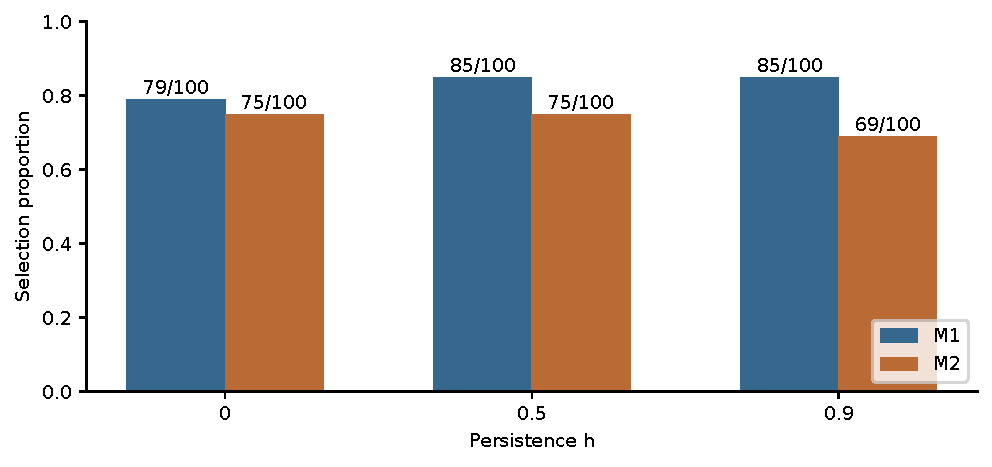
\includegraphics[width=\textwidth]{s02_completed_selection.pdf}\caption{Completed selection proportions under M1 and M2, each based on 100 paired forest units. The display is descriptive; saved custody checks and sampled raw validation passed.}\end{figure}

